%!TEX root =../cmbs4_scibook.tex 
%%%%%% CMB-S4 BSM Physics Chapter  %%%%%%%%%%%%%%%%

% This was created by Renee Hlozek from text in the inflation and neutrino sections

\chapter{Physics Beyond The Standard Model}

In addition to constraints on primordial parameters in the standard 6-parameter model, and a detection of (or upper limits on) the scalar-to-tensor ratio, CMB-S4 will yield unprecedented constraints on interesting physics beyond the standard picture. 

\section{Constraints on departures of Gaussian fluctuations}
\textbf{More is needed here to bring the non-Gaussian section to stand alone irrespective of the inflation chapter}

Perhaps of special interest for CMB-S4 are non-Gaussian signatures that would be expected in models of large field inflation. For example, in models in which the inflaton is an axion, there is only an approximate discrete shift symmetry. In that case instanton contributions to the potential and periodic bursts of particle or string production naturally lead to periodic features in the bispectrum. If moduli in the underlying string constructions do not evolve appreciably, instanton contributions lead to oscillations with a constant amplitude in the logarithm of $k$. In general, moduli evolve during inflation and cause a drift in the frequency and a scale-dependent amplitude~\cite{Flauger:2014ana}. At present, these shapes have not yet been constrained systematically. Often these contributions will lead to counter-parts in the power spectrum and are expected to be detected there first~\cite{Behbahani:2011it}, but this need not be the case~\cite{Behbahani:2012be}. A first attempt has been made~\cite{Ade:2015ava} to look for resonant and local features in the bispectrum and a more dedicated analysis is underway. Since features in the power spectrum and the bispectrum generally contain correlated parameters \cite{Achucarro:2010da,NonBDBispectrum2009,nonBDbispectrum2015,Flauger:2010ja} statistical methods have been developed to use the power of both the power spectrum and the bispectrum to further constrain models space \cite{Meerburg2015b,Moritz2016,Fergusson:2014hya}. Signatures of higher order massive spin fields \cite{Arkani-Hamed:2015bza,Chen:2015lza} would also lead to a bispectrum with decaying features, which will not be present in the power spectrum.  So a search for these more general shapes is well motivated. Using both $T$ and $E$-mode polarization, CMB-S4 will improve constraints by about of two compared to {\it Planck} as we will show in the next section. Bispectra containing at least one $B$ mode, will generally be much better constrained (currently there is no bound on such correlation functions) and will benefit from CMB-S4. We will consider two examples in the next section. 

More generally, one can divide the space of non-Gaussian inflationary models into those whose signals either (1) indicate fluctuations in degrees of freedom other than the inflaton, or (2) indicate non-trivial self-interactions of the effective inflaton fluctuation. Given the forecasted improvements from CMB-S4 over the {\it Planck}, it is unlikely that this instrument would uncover strong evidence of non-Gaussianity. However, since the {\it Planck} constraints have not ruled out $f_{\rm NL}\sim\mathcal{O}(1)$, even a hint of non-Gaussianity would be extremely interesting. Here we briefly review the physics in the two cases.

A detection of the widely studied local shape would have far reaching theoretical implications. A detection of this shape would rule out all models of single clock inflation \cite{Creminelli:2004yq}. In addition, such a signal would open the door to significant cosmic variance on all scales from coupling of fluctuations within our observed volume to any super-Hubble modes \cite{Nelson:2012sb,LoVerde:2013xka,Nurmi:2013xv}. Indeed, there would be room for a significant shift between the observed amplitude of scalar fluctuations (and so the observed $r$) and the mean value of fluctuations on much larger scales \cite{Bonga:2015urq}. Any scenario that predicts local non-Gaussianity together with fluctuations on scales much larger than our observed volume predicts a probability distribution for our observed $f_{\rm NL}^{\rm local}$, but many well-motivated scenarios also predict a small mean value. These include the simplest modulated reheating scenario \cite{Zaldarriaga:2003my} and ekpyrotic cosmology \cite{Lehners:2009ja}, both of which predict mean values of $f_{\rm NL}^{\rm local}\sim5$. 
Currently the strongest constraints on the local shape come from the {\it Planck} 2015 temperature and polarization analysis which finds $f_{\rm NL}^{\rm local} = 0.8 \pm 5.0$~\cite{Ade:2015ava}. A noise-free cosmic variance limited CMB experiment is expected to produce constraints on $f_{\rm NL}^{\rm local}$ with 1$\sigma$ error bars of about 3 \cite{Komatsu:2001rj}. Therefore the improvement expected of CMB-S4 over current limits is slightly less than a factor of two. This is not sufficient to reach the interesting theoretical threshold around $|f_{\rm NL}^{\rm local}|\lesssim 1$~\cite{Alvarez:2014vva}, but will still reduce the space of viable models or hint at a detection. CMB-S4 could, for example, provide hints for the mean level of non-Gaussianity expected from modulated reheating scenario or ekpyrotic cosmology at roughly $2\,\sigma$. The simplest curvaton scenario, which predicts $f_{\rm NL} = -5/4$ \cite{Lyth:2001nq}, will unfortunately be out of reach. Large-scale structure surveys (eg., \cite{Dore:2014cca}) may eventually achieve constraints $\sigma_{f_{\rm NL}}\sim\mathcal{O}(1)$. Those observations of the inhomogeneities in the late universe would be very complementary to the results of CMB-S4.

Equilateral and orthogonal shapes shapes arise in scenarios where the scalar perturbations sourced by inflaton fluctuations have non-trivial self interactions, and indicate an additional scale of particle physics, $M_{c_s}$ between $H$ and $M_p$. The amplitude of the non-Gaussianity typically scales as $(H/M_{c_s})^2$. Current constraints on the equilateral and orthogonal shapes are $f_{\rm NL}^{\rm equil} = -4 \pm 43$ and $f_{\rm NL}^{\rm ortho} = -26 \pm 21$, both (68\% CL)~\cite{Ade:2015ava}, which translates into $M_{c_s}>\mathcal{O}(10)H$. The improvements from CMB-S4 would further tighten existing constraints on the speed of sound during inflation and the strong coupling scale in single-clock models of inflation. In addition, the tighter constraints on the equilateral shape would constrain scenarios with secondary production of gravitational waves.



\subsection{Forecasts}

\begin{figure}[ht]
\centering
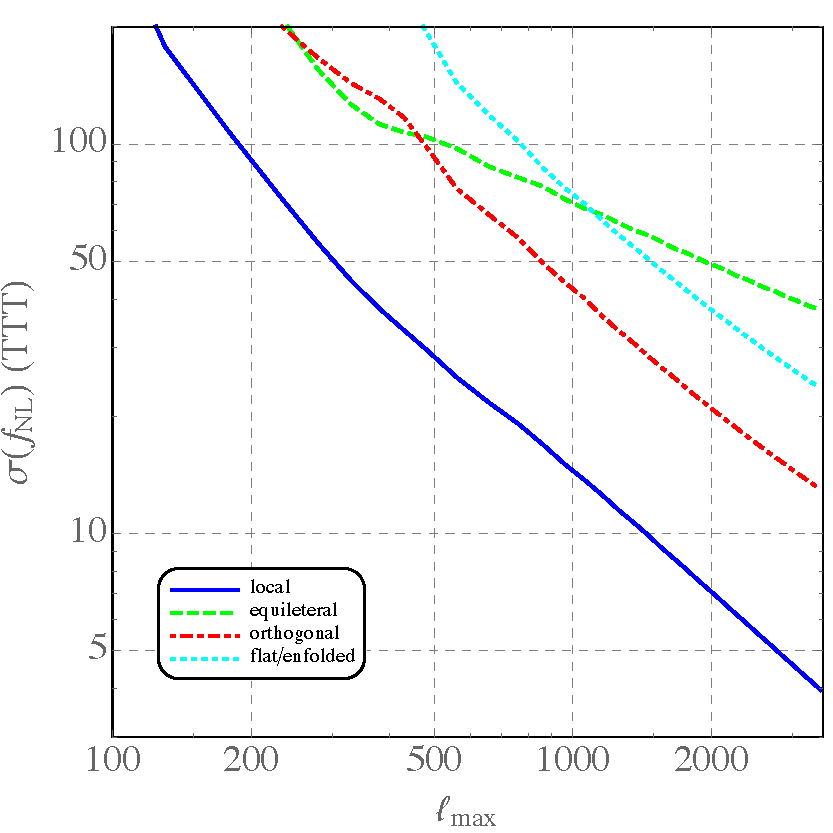
\includegraphics[width=0.4\textwidth]{Inflation/DeltaFNL_TTT}
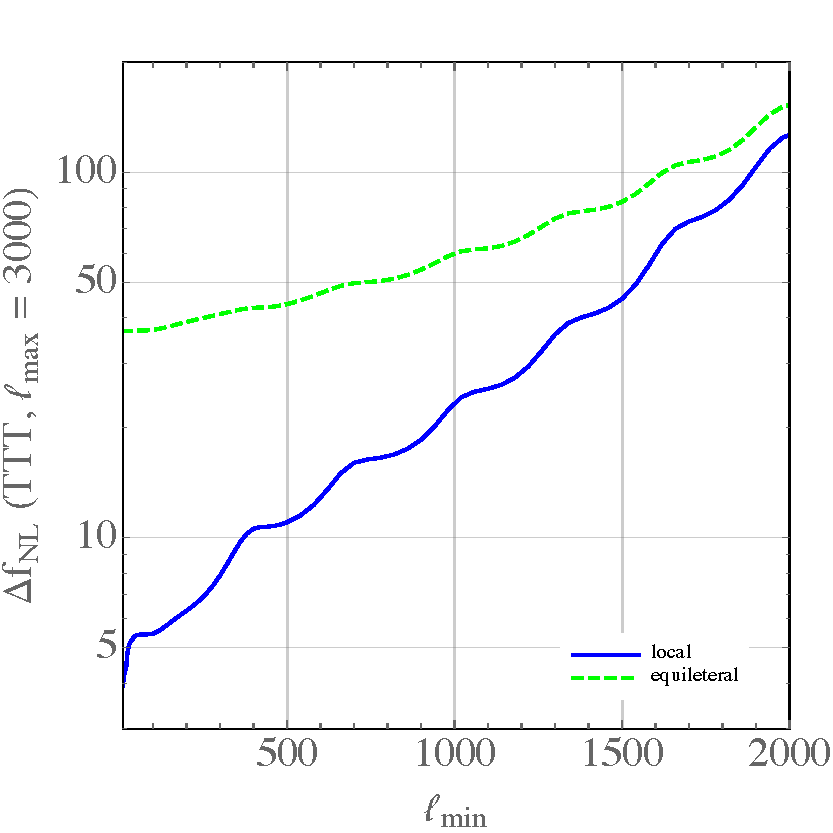
\includegraphics[width=0.415\textwidth]{Inflation/DeltaFNL_TTT_lmin}
\caption{Left: forecasts on the constraining power of CMB-S4 on 4 different types of non-Gaussianities as a function of $\ell_{\rm max}$. Right: Sensitivity of different types of non-Gaussianities on the minimum multipole. The local type non-Gaussianity benefits from having the lowest multipoles, while the other standard shapes saturate to a constant at low $\ell_{\rm min}$. }
\label{fig_fnlforecast}
\end{figure}

We forecast the constraints on non-Gaussianities from CMB-S4. We consider the most well motivated shapes; local, equilateral, orthogonal and enfolded. 
In Fig.~\ref{fig_fnlforecast} we show the constraints as a function of the maximum multipole on the left using the following configuration $f_{\rm sky} = 0.4$, $T$-noise = 1 $\mu$K-' and $E$-noise = $\sqrt{2}$ $\mu$K-' and a beam of $1$' and $\ell_{\rm min} = 30$. Local type non-Gaussianities benefit from large scales, and as much as $40\%$ of the signal is lost when considering the lowest multipoles as shown in Fig.~\ref{fig_fnlforecast} on the right. Ideally, large scale information from Planck \cite{Ade:2015ava} should be included to put the best constraints on non-Gaussianities. Including Planck low $\ell$ (using $f_{\rm sky} = 0.75$ \cite{Ade:2015ava} to determine the noise level, and $f_{\rm sky}=0.4$ for the maximal overlap) we can improve the forecasted bounds on local type non-Gaussianities by almost a factor of 2. Equilateral, enfolded and orthogonal non-Gaussianities are noy affected by not including the lowest multipoles. We summerize the results in Tab.~\ref{tab:fnl_forecast}. Note that our forecast, using Planck Blue Book\footnote{\url{http://www.rssd.esa.int/SA/PLANCK/docs/Bluebook-ESA-SCI(2005)1_V2.pdf}} values, deviate slightly from the actual bounds on non-Gaussianities obtained in Ref.~\cite{Ade:2015ava}. The expected factor of improvement over {\it Planck}-only is somewhere between 1.6 and 1.7 for all shapes considered.

% Requires the booktabs if the memoir class is not being used
\begin{table*}[t]\label{tab:fnl_forecast}
  \begin{center}
    \begin{tabular}{ | c || c | c | c | c |}
      \hline
      Type & Planck & CMB-S4 & CMB-S4 + low $\ell$ Planck & rel. improvement \\ \hline \hline
      local & $\sigma(f_{\rm NL}) = 4.6$ & $\sigma(f_{\rm NL}) = 3.9$ &  $\sigma(f_{\rm NL}) = 2.7$ & 1.7\\ \hline 
      equilateral &  $\sigma(f_{\rm NL}) = 40.5$ & $\sigma(f_{\rm NL}) = 24$ &  $\sigma(f_{\rm NL}) = 24$ & 1.7\\ \hline 
      orthogonal &  $\sigma(f_{\rm NL}) = 20.2$ & $\sigma(f_{\rm NL}) = 12.3$ &  $\sigma(f_{\rm NL}) = 12.3$ & 1.6\\ \hline 
      flat &  $\sigma(f_{\rm NL}) = 35$ & $\sigma(f_{\rm NL}) = 21.8$ &  $\sigma(f_{\rm NL}) = 21.8$ & 1.6\\ \hline 
    \end{tabular}
  \end{center}
  \caption{Forecasted constraints on several well motivated non-Gaussian shapes using $T$ and $E$ modes. {\it Planck} forecast is based on Blue Book values, with $f_{\rm sky} = 0.75$. CMBS-4 has $\ell_{\rm min} = 30$, which mostly affects local type non-Gaussianities. The table shows we need to include low $\ell$ information from {\it Planck} for local type non-Gaussianities.}
  \label{default}
\end{table*}

\begin{figure}[ht]
\centering
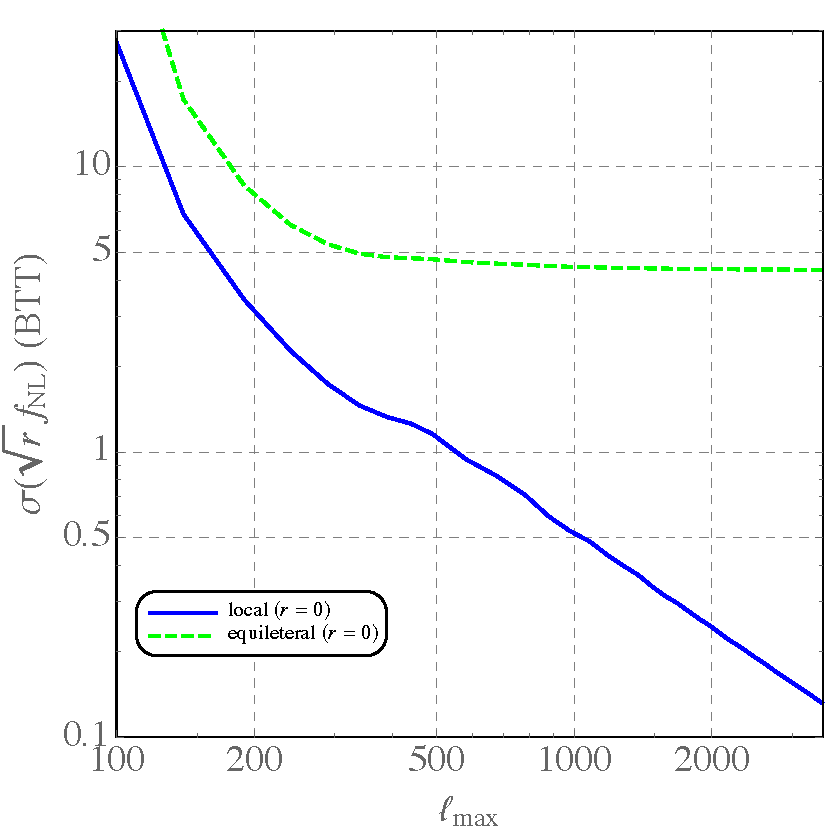
\includegraphics[width=0.45\textwidth]{Inflation/DeltaFNL_BTT_no_r}
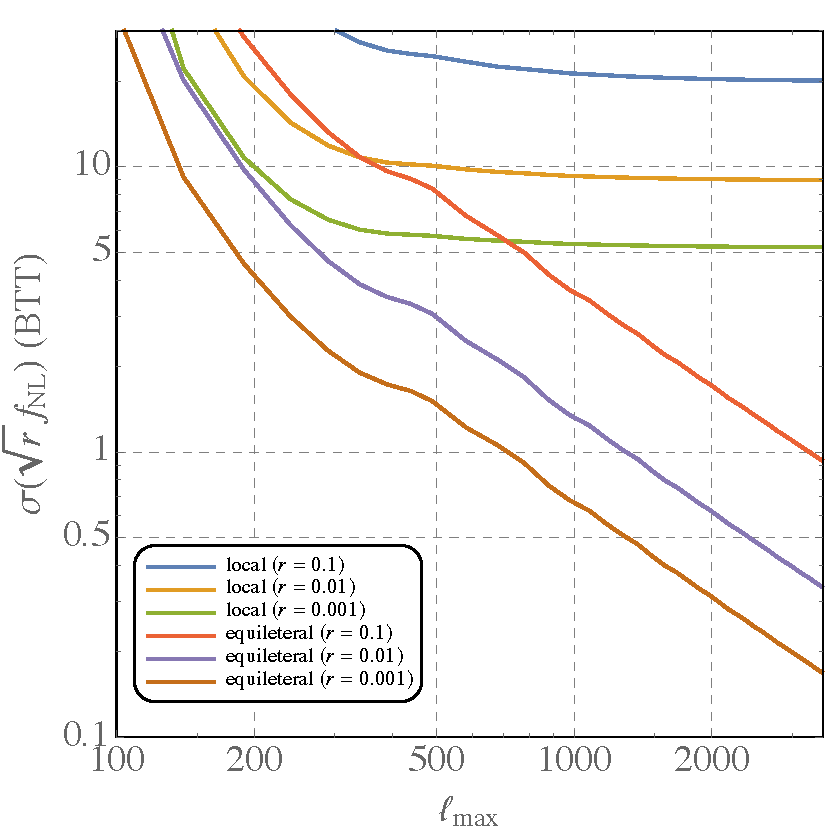
\includegraphics[width=0.45\textwidth]{Inflation/DeltaFNL_BTT_with_r}
\caption{Left: Noise dominated $B$ modes. Forecasts on the constraining power of CMB-S4 on two types of $\langle h \zeta \zeta\rangle$ non-Gaussianities as a function of $\ell_{\rm max}$ using $\langle BTT\rangle$. Right: the effect of cosmic variance in $B$.  }
\label{fig_fnlforecastBTT}
\end{figure}

Next, we determine the improvements as function of a fixed effort with $f_{\rm sky} = 0.4$ corresponding to noise of 1 $\mu$K-arcmin. 

Correlators including at least one $B$ mode will benefit from the improved sensitivity of $B$ modes significantly. We define \cite{Meerburg2016}
\begin{equation}
\langle \zeta(\vec{k}_1)\zeta(\vec{k}_2)h^{\pm}(\vec{k}_3) \rangle = (2\pi)^3  \delta^{(3)} \left(\sum_{n=1}^3\vec{k}_n\right) \mathcal{B}(k_1,k_2,k_3) e_{ab}^{\mp}(\vec{k}_3)\hat{k}_1^a \hat{k}_2^b, 
\end{equation}
with 
\begin{equation}
\mathcal{B}(k_1,k_2,k_3)= 16 \pi^4 A_s^2 \sqrt{r}f_\mathrm{NL}^{h\zeta\zeta} F(k_1,k_2,k_3)
\end{equation}
and $e_{ab}^{\mp}$ the transvere traceless polarization tensor. 
In the simplest model of inflation $f^{h \zeta \zeta}_{\rm NL} = \sqrt{r}/16$ \cite{Maldacena:2002vr,Maldacena:2011nz} which realistically is undetectable small. As mentioned before in Sec.~\ref{subsubsec:Interactions}, a measurement if this correlation would be an immediate indication of some deviation from the simple inflationary paradigm and as such would provide valuable information. The coupling above can be constrained using any type of correlation that contains one $B$ mode, e.g. $\langle BTT \rangle$ or $\langle BEE\rangle$. For $F$ we use local and equilateral shaped triangles and forecast the constraint on the amplitude in Fig.~\ref{fig_fnlforecastBTT} for $\langle BTT\rangle$. We anticipate similar constraints for $\langle BTE\rangle $ and $\langle BEE\rangle$. 

\begin{figure}[ht]
\centering
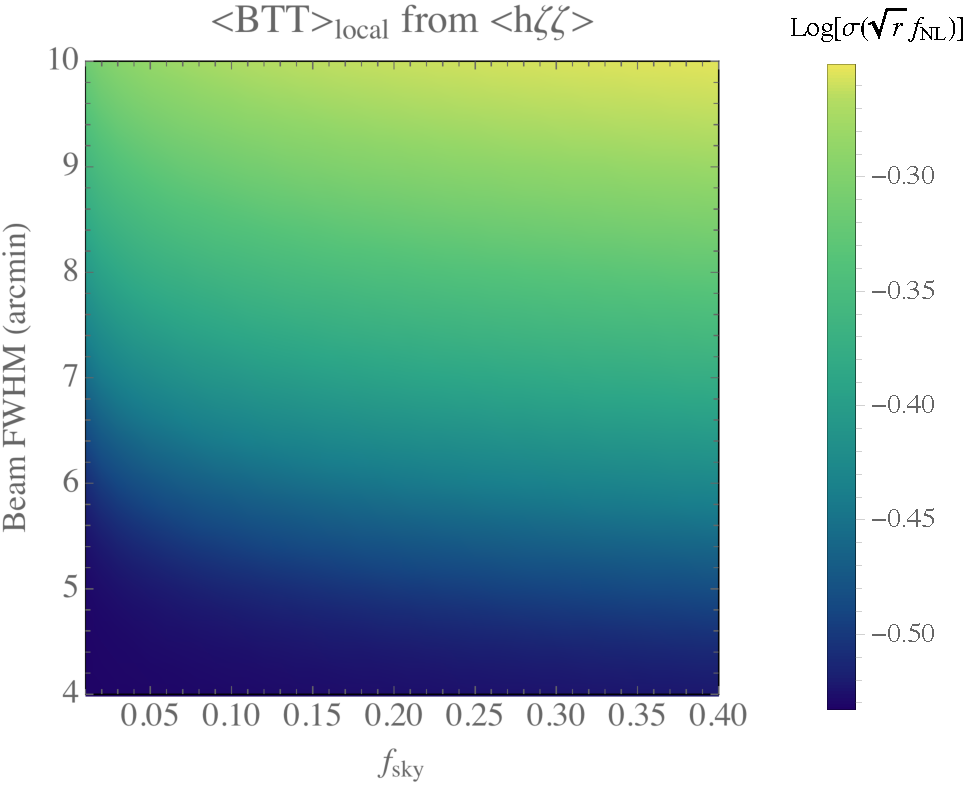
\includegraphics[width=0.48\textwidth]{Inflation/FixedEffortBTTlocal}
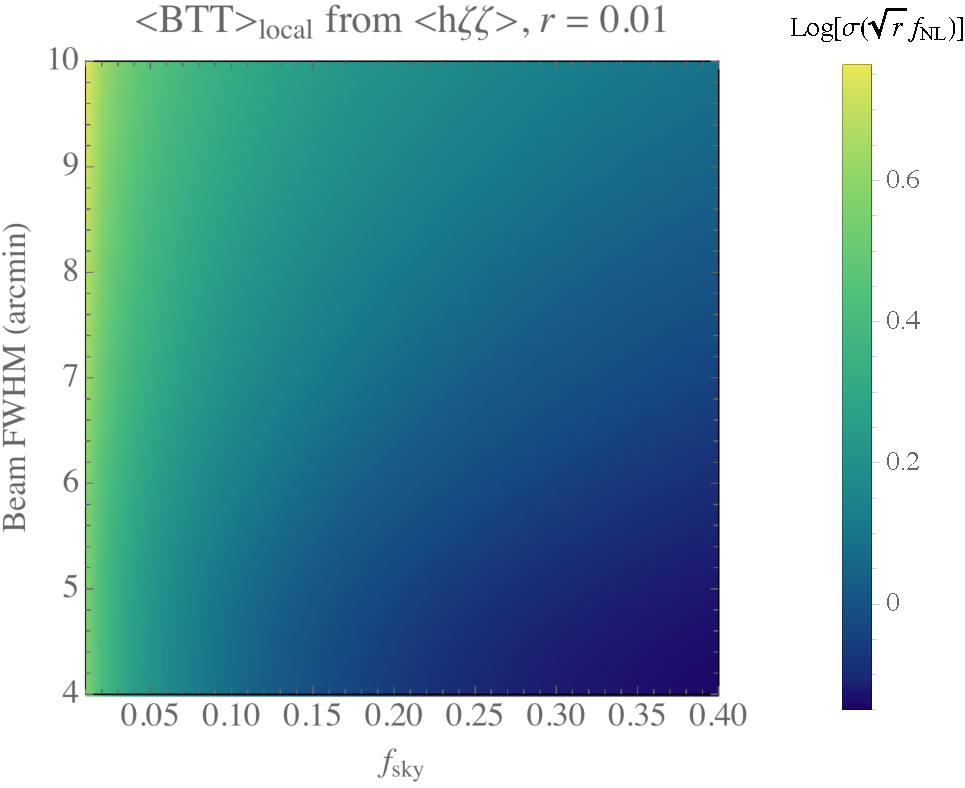
\includegraphics[width=0.48\textwidth]{Inflation/FixedEffortBTTlocalr}
\caption{Left: Fixed effort density plot for local type $BTT$. Left, the effect of beam and $f_{\rm sky}$ variation in noise dominated $B$ mode. $f_{\rm sky}$ has very little effect, as it is cancelled by the $f_{\rm sky}$ associated with the masking of the total map. Right: adding a signal changes this picture, since the cancellation no longer happens for $r > 0.001$ (i.e. when CMB-S4 becomes cosmic variance limited). A larger sky fraction benefits cosmic variance limited $\langle BTT\rangle$. }
\label{fig_BTTlocalfixedeffort}
\end{figure}

We consider two scenarios; one in which the $B$ modes are noise dominated and one in which they are cosmic variance limited by a future detection of $r$. For a local shape primordial bispectrum the error decreases as you decrease the beam. The signal is dominated by large angle $B$ modes correlated with small angle $T$ modes as was pointed out in \cite{Meerburg2016}. An equilateral component from the $\langle BTT\rangle$ correlation function suffers from the decaying tensor modes, which are negligible for $\ell_B > 500$. After this, no equilateral triangles can be constructed and the error saturates. The effect is that equilateral type non-Gaussianities are almost insensitive to beam size. For both shapes, in a scenario where $B$ modes are noise dominated, $f_{\rm sky}$ have very little effect. 

On the right we show what happens when $B$ gets a primordial component; the take away message is that only if $r < 0.001$  CMB-S4 noise dominates cosmic variance. 

In addition we consider fixed effort. We show the results in Fig.~\ref{fig_BTTlocalfixedeffort} and \ref{fig_BTTequilfixedeffort}. We find that $BTT$ is practically insensitive to $f_{\rm sky}$ as long as $B$ modes are noise dominated. For $r = 0.001$ and above a larger sky fraction helps constrain $\langle BTT \rangle$. 

\begin{figure}[ht]
\centering
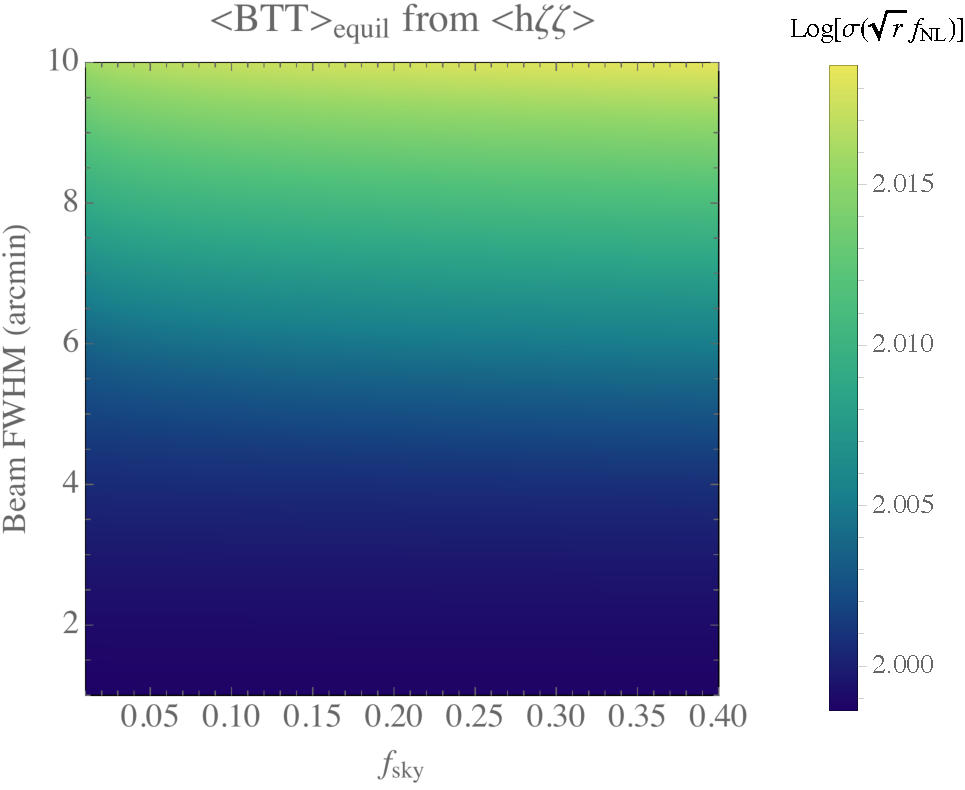
\includegraphics[width=0.48\textwidth]{Inflation/FixedEffortBTTequil}
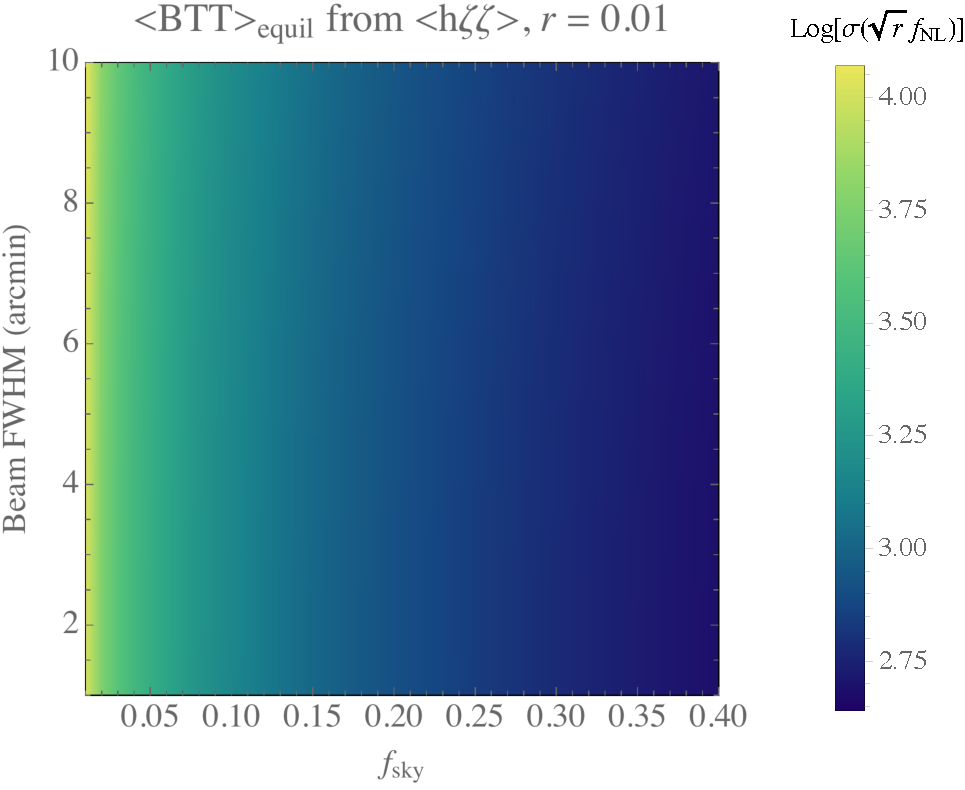
\includegraphics[width=0.48\textwidth]{Inflation/FixedEffortBTTequilr}
\caption{Left: Fixed effort density plot for equilateral type $BTT$. Similar to local type bispectra, a larger sky fraction benefits cosmic variance limited $\langle BTT\rangle$. }
\label{fig_BTTequilfixedeffort}
\end{figure}
%In models with a single clock, the symmetry breaking pattern underlying inflation guarantees that the fluctuations are governed by the action
%\begin{equation}
%S=\int\,d^4 x \sqrt{-g}\left[-\frac{M_p^2 \dot{H}}{c_s^2}\left(\dot{\pi}^2-c_s^2\frac{(\partial_i\pi)^2}{a^2}\right)+M_p^2 \dot{H}\left(1-\frac{1}{c_s^2}\right)\left(\dot\pi^3-\dot\pi\frac{(\partial_i\pi)^2}{a^2}\right)+M_3^4\dot\pi^3+\dots\right]\,,
%\end{equation}
%where at leading order $\zeta=H\pi$ and the omissions represent terms higher order in fields, derivatives, or both. In the presence of an approximate continuous shift symmetry, the coefficients in this action are approximately constant in time and there are only two linearly independent shapes. 
%Current constraints on the equilateral and orthogonal shapes are $f_{\rm NL}^{\rm equil} = -4 \pm 43$ and $f_{\rm NL}^{\rm ortho} = -26 \pm 21$, both (68\% CL)~\cite{Ade:2015ava}. Because of its high angular resolution, CMB-S4 can improve these constraints by about a factor two which would further tighten existing constraints on the speed of sound during inflation and the strong coupling scale in single-clock models of inflation. In addition, the tighter constraints on the equilateral shape would constrain scenarios with secondary production of gravitational waves.

{\color{blue} Any one care to work this out more:} 
Higher order statistics encode further information about particle content and interactions. The relative amplitude of certain limits of the trispectrum (the momentum space 4-point function) and of the trispectrum can also reveal whether there may be multiple sources contributing to the primordial fluctuations (and both may be different from the fluctuations of the inflaton). {\bf more...}


%In the modulated reheating scenario, the field which drives inflation $\phi$ decays to the particles of the standard model with a rate $\gamma$ which is determined by the value of a second field $\sigma$ which remains light throughout inflation. The quantum fluctuations in $\sigma$ result in a spatially modulated reheating surface resulting in the curvature perturbations that we observe in the CMB and large scale structure. The process by which the fluctuations in the light field are converted into curvature fluctuations naturally results in local non-Gaussianity given by $f_{\rm NL} = 5(1-\Gamma \Gamma^{\prime\prime}/\Gamma^{\prime2})$, where this formula holds in the case that $\phi$ oscillates about a quadratic minimum after inflation and the fluctuations in $\phi$ make a negligible contribution to the observed power spectrum.

%This can be contrasted with the simplest curvaton scenario, where a scalar field $\sigma$ which remains light during inflation comes to dominate the energy density of the universe after the field which drives inflation $\phi$ decays. The fluctuations in the energy density of $\sigma$ then determine the curvature perturbations that are observed today. The local non-Gaussianity in this simple model is predicted to be $f_{\rm NL} = -5/4$ \cite{Lyth:2001nq}, which is unfortunately a few times smaller than the expected error bar from CMB Stage-IV.

%In the absence of a detection, however, it is important to ask what can be learned from improved constraints on $f_{\rm NL}$. Though not firm, nor entirely robustly defined, it can be argued that a natural theoretical threshold where qualitatively new general conclusions about the physics of the early universe can be drawn would come from constraints on $f_{\rm NL}<\mathcal{O}(1)$, see for example [1412.4671] for a detailed discussion. In order to achieve this level of constraint, it seems necessary to move beyond the cosmic microwave background to study other data sets, such as large scale structure. Despite the fact that CMB Stage-IV is not expected to reach this threshold, it is worth asking what can be gleaned from an improved constraint on $f_{\rm NL}$ from the CMB.

\section{Spatial Curvature}

Despite the fact that inflation drives the spatial curvature to zero at the level of the background evolution, it predicts small, but non-zero curvature for a typical observer. The curvature measured in a Hubble patch receives contributions from long wavelength perturbations and is expected to be $|\Omega_k|<10^{-4}$. A measurements of $\Omega_k$ exceeding this expectation would contain important information about the process responsible for inflation. In particular, if $|\Omega_k|$ is found to be considerably larger than this value, it would tell us that the inflaton was not slowly rolling when scales slightly larger than our observable horizon exited the horizon. Furthermore, observations of large negative $\Omega_k$ would falsify eternal inflation, while observation of positive and large $\Omega_k$ would be consistent with false vacuum eternal inflation~\cite{Guth:2012ww,Kleban:2012ph}.

Current constraints on this parameter from the CMB alone are $\Omega_k= 0.005^{+0.016}_{-0.017}$. Including baryon acoustic oscillation (BAO) data tightens the bound to $\Omega_k=0.000\pm0.005$. CMB-S4 is expected to constrain spatial curvature at a level of $\sigma(\Omega_k)\approx 10^{-3}$. A detection at this level would have profound implications for the inflationary paradigm. 

\section{Isocurvature}
Measurements of CMB temperature/polarization power spectra indicate that the primordial initial conditions are adiabatic, that is, spatial entropy fluctuations vanish:
\begin{align}
S_{i \gamma}\equiv \frac{\delta n_{i}}{n_{i}}-\frac{\delta n_{\gamma}}{n_{\gamma}} =0.\end{align} The species label $i$ can denote baryons, cold dark matter (CDM), or neutrinos. Number densities are denoted by $n_{i}$ and perturbations in them by $\delta n_{i}$.

Adiabatic perturbations are produced in models where the initial perturbations in all species are seeded by the inflaton. If fluctuations are also sourced by a second field, the initial conditions are a mixture of adiabatic and entropy (a.k.a isocurvature) perturbations, for which $S_{i\gamma}\neq 0$. These initial conditions determine the acoustic peak structure and large-scale amplitude of CMB anisotropies, as well as large-scale structure statistics \cite{Bond:1984fp,Kodama:1986fg,Kodama:1986ud,Hu:1994jd,Moodley:2004nz,Bean:2006qz}. Observations can thus probe the number of fields during inflation. 
\label{sec:isosec}
Each species can carry isocurvature perturbations in its density (e.g. Refs~\cite{Bucher:1999re,Bucher:2004an,Moodley:2004nz}).\footnote{Neutrinos can also carry velocity isocurvature, but this mode is not well motivated in inflationary models.} Indeed, the modes of the perturbation evolution equations correspond to adiabatic, CDM density isocurvature (CDI), baryon density isocurvature (BDI), neutrino density isocurvature (NDI), and neutrino velocity isocurvature (NVI) initial conditions. 

\begin{figure*}[htbp!]
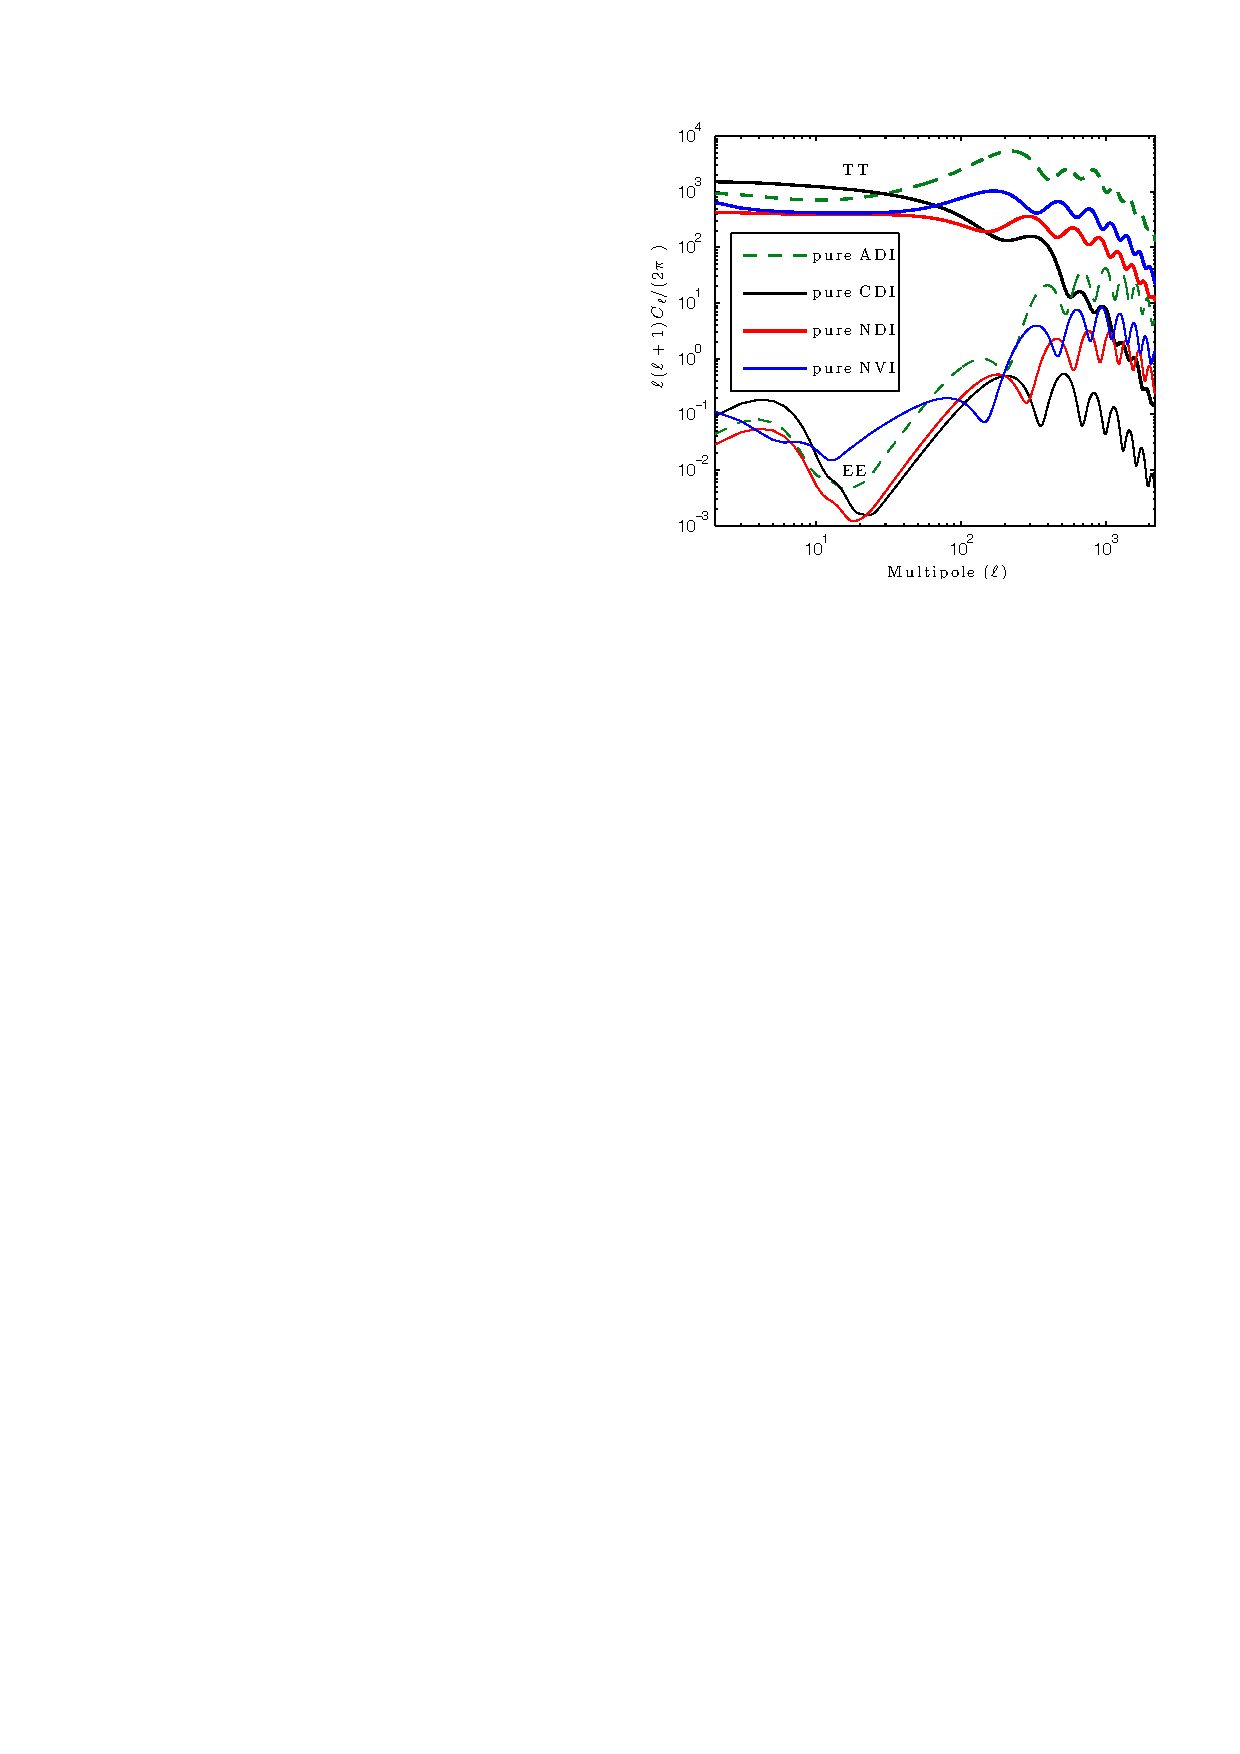
\includegraphics[width=0.5\textwidth, trim={0 10 0 0},clip]{Inflation/iso_schematic.pdf} 
 \caption{CMB isocurvature power spectra $C_{l}^{\rm TT}$ (solid) and $C_{l}^{\rm EE}$ (dashed) for equal primordial $P_{\zeta\zeta}(k)$  isocurvature perturbations. \textbf{Figure appropriated from Planck inflation paper. To be replaced by our own figure.}
\label{fig:iso_schematic}}
\end{figure*} 

Data from WMAP \cite{dunkley09}, \textit{Planck} \cite{Ade:2015lrj}, and other experiments \cite{Enqvist:2000hp,MacTavish:2005yk} indicate that perturbations are predominantly adiabatic. The limits can stated in terms of the fractional primordial power in each isocurvature mode:\begin{equation}
\beta\equiv \frac{P_{S_{i\gamma}}(k)}{P_{S_{i\gamma}}(k)+P_{\zeta\zeta}(k)}.
\end{equation}
The current CMB limits (allowing one isocurvature mode at a time) are shown in Table \ref{table:fisher_model_independent}, along with a forecast of CMB-S4 sensitivity.\footnote{All forecasts in the isocurvature section are produced using Fisher-matrix techniques.} In Table. \ref{table:fisher_model_independent}, ``correlated'' refers to totally correlated or anti-correlated (with $\zeta$) isocurvature perturbations. All results are quoted at a fiducial $k=0.05~{\rm Mpc}^{-1}$. Limits to BDI perturbations are not separately listed, as at linear order they are indistinguishable from CDI perturbations \cite{Gordon:2002gv,Lewis:2002nc,Lewis:2007kz,Gordon:2009wx}. CMB-S4 could improve on these limits by a factor of $2-5$, as shown in Table. \ref{table:fisher_model_independent}.

\begin{table}
\begin{center}
\begin{tabular}
{lcccc}\hline \hline {\rm Mode} &  $ \beta $ (\emph{Planck}, uncorrelated )&$ \beta$(CMB-S4, uncorrelated)&  $ \beta $ (\emph{Planck}, correlated )&$ \beta$(CMB-S4, correlated)\\ 
\hline \\
CDI & $\leq 0.04$&$0.008$&$\leq0.001$&$4\times 10^{-4}$\\
NDI &  $\leq 0.01$ &$XX$&$XX$&$XX$\\
NVI &  $\leq 0.04$&$XX$&$XX$&$XX$\\
\\ \hline \hline 
\end{tabular}
\caption{Constraints (from \emph{Planck} \cite{Ade:2015lrj}) TT+BAO+LowP data vs. CMB-S4 sensitivity to fractional primordial isocurvature power $\beta$ ($95\%$ C.L.) in various modes for uncorrelated/correlated isocurvature modes.\textbf{Numbers to be finalised based on results of Fisher forecast efforts.}
\label{table:fisher_model_independent}}
\end{center}
\end{table} 

\subsection{The Curvaton Scenario}
One alternative to single-field models is the curvaton scenario, in which a sub-dominant second field $\sigma$ acquires vacuum fluctuations during inflation, becomes more important later, sources $\zeta$, and then decays \cite{Mollerach:1989hu,Mukhanov:1990me,Moroi:2001ct,Lyth:2001nq,Lyth:2002my}. Curvaton candidates include sneutrinos, string moduli, and others \cite{Postma:2002et,Kasuya:2003va,Ikegami:2004ve,Mazumdar:2004qv,Allahverdi:2006dr,Papantonopoulos:2006xi,Mazumdar:2010sa,Mazumdar:2011xe}. Depending on whether a species $i$ (or its quantum numbers ) is produced by, before, or after curvaton decay, perturbations in $i$ are offset from $\zeta$, leading to isocurvature perturbations: \cite{Lyth:2001nq,Lyth:2002my,Gordon:2002gv}

\begin{eqnarray}
S_{i \gamma}=\left\{\begin{array}{ll}-3\zeta-3(\zeta_{\gamma}-\zeta),&\mbox{if $i$ is produced before $\sigma$ decay,}\\3\left(\frac{1}{r_{D}}-1\right)\zeta-3(\zeta_{\gamma}-\zeta),&\mbox{if $i$ is produced by $\sigma$ decay},\\ -3(\zeta_\gamma-\zeta),&\mbox{if $i$ is produced after $\sigma$ decay},\end{array}\right.\label{eq:strew}.
\end{eqnarray} Here $\zeta_{i}$ is the density perturbation in $i$ on surfaces of constant curvature. The parameter $r_{\rm D}$ is the fractional energy density in the curvaton when it decays. 

The mixture of isocurvature modes is determined by whether or not baryon number, lepton number, and CDM are produced before, by, or after curvaton decay. Curvaton-type isocurvature is distinct from axion isocurvature, as it is correlated (or anti-correlated) $\zeta$. If lepton number is produced by curvaton decay, the lepton chemical potential $\xi_{\rm lep}$ is important in setting the amplitude of NDI modes \cite{Lyth:2002my,Gordon:2003hw,DiValentino:2011sv}:
\begin{equation}
S_{\nu \gamma}=
-\frac{135}{7}\left(\frac{\xi_{\rm lep}}{\pi}\right)^2\zeta_{\gamma}.\end{equation}
There are $27$ distinct curvaton decay scenarios, as baryon number, lepton number, and CDM could each be produced before, by, or after curvaton decay. Viable models are those in which one of baryon number or CDM is produced by curvaton decay, and those in which \textit{both} baryon number and CDM are produced after curvaton decay. For curvaton-decay scenarios, we use the notation ($b_{x}$, $c_{y}$, $L_{z}$), where $x\in ({\rm before, by, after})$. Here $b$ denotes baryon number, $c$ denotes CDM, and $L$ denotes lepton number. For example, $(b_{\rm before}, c_{\rm by}, L_{\rm by})$ is a model in which baryon number is produced before curvaton decay, CDM by curvaton decay, and lepton number by curvaton decay.

Current isocurvature limits favor values of $r_{\rm D}\simeq 1$, except for models in which baryon number is produced by curvaton decay and CDM before (or vice versa), which favor central values of $r_{\rm D} \simeq 0.16$ ($r_{\rm D} \simeq 0.84$). 

The current limits \cite{Smith/Grin:2015} to $r_{\rm D}$ are shown in Table \ref{limits_rd}, along with a forecast of CMB-S4's sensitivity to $r_{\rm D}$ via isocurvature. The dramatic improvement in the $(b_{\rm by},c_{\rm before},L_{\rm by})$ and $(b_{\rm before},c_{\rm by},L_{\rm by})$ scenarios because of the accompanying NDI perturbations. One unusual case is the $(b_{\rm after},c_{\rm after}, L_{y_{\rm L}})$ scenario. Here isocurvature just constrains the degenerate combination \cite{Smith/Grin:2015} $\chi_{\rm D} \equiv \left\{1+\xi_{\rm lep}^2/(\pi^2) \left(1/r_D -1\right)\right\}^{-1}$, while the independent constraint to $\xi_{\rm lep}^{2}$ is driven by the $N_{\rm eff}$ limit from the CMB.

\begin{table}
\begin{center}
\begin{tabular}
{lcc}\hline \hline {\rm scenario} &  $ \Delta r_D/r_{D}^{\rm adi}$ (\emph{Planck})&$ \Delta r_D/r_{D}^{\rm adi}$(CMB-S4)\\ 
\hline \\
$(b_{\rm by},c_{\rm before},L_{y_{L}})$ & $0.03$&$0.005$\\
$(b_{\rm before},c_{\rm by},L_{y_{L}})$ &  $0.01$ &$0.004$\\
$(b_{\rm by},c_{\rm after},L_{y_{L}})$ &  $0.04$&$0.01$\\
$(b_{\rm after},c_{\rm by},L_{y_{L}})$ & $0.008$&$0.002$\\
$(b_{\rm by},c_{\rm by},L_{y_{L}})$ &  $0.007$&$0.002$\\\hline \hline \\ & $\Delta \chi_{\rm D}/\chi_{\rm }^{\rm adi}$ (\emph{Planck})&$\Delta \chi_{\rm D}/\chi_{\rm }^{\rm adi}$ (CMB-S4) \\\hline \\
$(b_{\rm after},c_{\rm after},L_{y_{L}})$ & $0.003$&$0.0004$\\
\\ 
\end{tabular}
\caption{Isocurvature constraints on $r_D$ ($95\%$ C.L.) using \textit{Planck} TT+BAO+LowP data \cite{Smith/Grin:2015} in viable curvaton decay-scenarios, and Fisher forecasts for CMB-S4 sensitivity. \textbf{Numbers to be finalised based on the final Fisher forecasts as part of larger forecast effort}.
\label{limits_rd}}
\end{center}
\end{table}

\begin{table}
\begin{center}
\begin{tabular}
{lcc}\hline \hline {\rm scenario} &  $\Delta \xi^{2}_{\rm lep}$ (\emph{Planck})&$\Delta \xi^{2}_{\rm lep}$ (CMB-S4) \\ 
\hline \\
$(b_{\rm by},c_{\rm before},L_{\rm by})$ &$0.02$ &$0.002$\\
$(b_{\rm before},c_{\rm by},L_{\rm by})$ &$0.4$  & $0.04$\\
$(b_{\rm by},c_{\rm after},L_{\rm by})$ &$0.3$  &$0.04$\\
$(b_{\rm after},c_{\rm by},L_{\rm by})$ & $0.3$&$0.04$\\
$(b_{\rm by},c_{\rm by},L_{\rm by})$ & $0.3$ & $0.04$\\
$(b_{\rm after},c_{\rm after},L_{\rm by})$ & $0.3$ & $0.04$\\
\\ \hline \hline 
\end{tabular}
\caption{Isocurvature constraints on $\xi_{\rm lep}^{2}$ ($95\%$ C.L.) using \textit{Planck} TT+BAO+LowP data \cite{Smith/Grin:2015} in viable curvaton decay-scenarios where lepton number is generated by curvaton decay, and Fisher forecasts for CMB-S4 sensitivity.\textbf{Numbers to be finalised in forecasting effort.}
\label{limits_xilep}}
\end{center}
\end{table}

Depending on the scenario, forecasting shows that the S4 sensitivity to curvaton-sourced isocurvature should improve by a factor of $2-4$ on current limits. In models with nearly-canceling CDM and baryon isocurvature perturbations, S4 limits to neutrino isocurvature drive an improvement in the sensitivity to the lepton asymmetry from $\Delta \xi_{\rm lep}^{2}\simeq 0.015$ to $\Delta \xi_{\rm lep}^{2}\simeq 0.003$. This dramatic improvement would make CMB limits comparably sensitive to BBN probes $\xi_{\rm lep}^{2}$ (for this decay scenario).

If baryon number/CDM are produced by/before curvaton decay (or vice versa), a relative large compensated isocurvature perturbation (CIP) is produced between the baryons and CDM, that is
\begin{equation}
S_{bc}=\frac{\delta n_{\rm b}}{n_{\rm b}}-\frac{\delta n_{\rm c}}{n_{\rm c}}\neq 0.
\end{equation} Curvaton-generated CIPs are proportional to $\zeta$, $S_{\rm bc}=A\zeta$, where $A\simeq 17$ [$A\simeq -3$] in the $(b_{\rm by}, c_{\rm before}, L_{\rm z})$ [$(b_{\rm before}, c_{\rm by}, L_{\rm z})$] scenario. For CIPs, the initial relative densities of baryons and CDM vary, but with no additional overall matter or radiation density fluctuation.
CIPs are relatively unconstrained at the level of the CMB power-spectrum (see Ref. \cite{Munoz:2015fdv} for an exception), but would induce non-Gaussianities in the CMB \cite{Grin:2011nk,Grin:2011tf,Grin:2013uya,He:2015msa}. As with weak gravitational lensing \cite{Hu:2001kj}, the CIP field $\Delta(\hat{n})$ can be reconstructed using CMB data. We find that at S4 sensitivity \cite{He:2015msa}, the threshold for a $95\%$ C.L. detection is $A\simeq 10$, and so a CIP test of the $(b_{\rm by}, c_{\rm before}, L_{\rm z})$ scenario is within reach of CMB-S4. This is a vast improvement over \emph{Planck} sensitivity, which at $95\%$ C.L. is $A\simeq 43$. Uncorrelated CIPs are less  motivated theoretically. Updating the analysis of Ref. \cite{He:2015msa} with current parameters \cite{Ade:2015lrj} and CMB-S4 specifications, we find that the sensitivity of CMB-S4 to a scale-invariant (SI) angular power spectrum of uncorrelated CIPs is $\Delta_{\rm cl}=0.003$ at the $95\%$ C.L. detection limit. Here $\Delta_{\rm cl}$ is the r.m.s. CIP amplitude on cluster scales. This is a vast improvement over the upper limit of $\Delta_{\rm cl}\leq 0.077$ from WMAP \cite{Grin:2013uya}, or the forecasted Planck \cite{Ade:2015lrj} (including polarization) sensitivity of $\Delta_{\rm cl}\leq 0.015$ \cite{He:2015msa}.


%We now focus on two isocurvature scenarios, axion dark matter and the curvaton %model, which produce uncorrelated and correlated isocurvature pertrubrations, %respectively.


\section{Constraints on Axion-like particles}
The QCD axion and other axion-like particles (ALPs), if stable on cosmological timescales, can contribute to the DM density. Along with thermal WIMPs, they are a well-motivated DM candidate (see Ref.~\cite{Marsh:2015xka} for a recent review).

We discuss below both constraints on axion isocurvature and axion-photon mixing. Constraints on the axion energy density and its contribution to the total dark matter density of the universe are described in section DM/DE \textbf{[Perhaps these constraints need to move here too]}

\subsection{Axion Isocurvature}

A key axion parameter is the symmetry breaking scale, $f_a$. If $H_I/2\pi<f_a$, the axion DM acquires \emph{uncorrelated isocurvature perturbations} (e.g. Refs.~\cite{Axenides:1983hj,Fox:2004kb,Hertzberg:2008wr}).\footnote{We ignore the case where $H_I/2\pi>f_a$, since no isocurvature initial conditions are excited. The limit $r_{0.05}<0.12$ implies that isocurvature is produced if $f_a>1.8\times 10^{13}\text{ GeV}$. This accounts for the QCD axion in the ``anthropic'' window (roughly half of the allowed range of $f_a$ on a logarithmic scale), axions with GUT scale decay constants (such as string axions~\cite{Svrcek:2006yi,Arvanitaki:2009fg}) and axions with lower $f_a$ in models of low-scale inflation.} The uncorrelated CDM isocurvature amplitude is bounded by \emph{Planck} to be $A_I/A_s<0.038$ at 95\% C.L.~\cite{Ade:2015lrj}. We performed a forecast for CMB-S4: the isocurvature limit will be improved by a factor of approximately five compared to \emph{Planck}, allowing for detection of axion-type isocurvature at 2$\sigma$ significance in the region $0.008<A_I/A_s<0.038$.

The axion isocurvature amplitude is:
\begin{equation}
A_I = \left(\frac{\Omega_a}{\Omega_d}\right)^2\frac{(H_I/M_{\rm pl})^2}{\pi^2(\phi_i/M_{\rm pl})^2} \, .
\label{eqn:iso_amplitude}
\end{equation}
The initial axion displacement, $\phi_i$, fixes the axion relic abundance such that $\Omega_a=\Omega_a (\phi_i,m_a)$~\cite{Preskill:1982cy,Abbott:1982af,Dine:1982ah,Turner:1983he,Steinhardt:1983ia,Marsh:2010wq}. Thus, if the relic density and mass can be measured by independent means, \emph{a measurement of the axion isocurvature amplitude can be used to measure the energy scale of inflation, $H_I$}

If the QCD axion is all of the DM, axion direct detection experiments can be used in conjunction with CMB-S4 to probe $H_I$ in the range
\begin{equation}
 2.5\times 10^6\lesssim H_I/\text{GeV}\lesssim 4\times 10^9\, 
\text{(QCD axion + direct detection)}\, \,
\end{equation}
This is demonstrated in Fig.~\ref{fig:qcd_isocurvature} (left panel) for the case of ADMX~\cite{Asztalos:2009yp} (in operation), and CASPEr~\cite{Budker:2013hf} (proposed), where we have used the standard formulae relating the QCD axion mass and relic abundance to the decay constant (e.g. Ref.~\cite{Fox:2004kb}).\footnote{In simple models of inflation, the high-$f_a$ QCD axion is incompatible with detection of tensor modes~\cite{Fox:2004kb,Hertzberg:2008wr,Visinelli:2014twa,Marsh:2014qoa,Visinelli:2014twa}, although non-standard cosmic thermal histories of PQ breaking mechanisms can lift constraints , e.g. \cite{Higaki:2014ooa,Fairbairn:2014zta,Nomura:2015xil}.} \emph{Combining axion DM direct detection with CMB-S4 isocurvature measurements allows a unique probe of low-scale inflation, inaccessible to searches for tensor modes.}

\begin{figure*}[htbp!]
\begin{center}
$\begin{array}{@{\hspace{-0.8in}}c@{\hspace{+0.2in}}c@{\hspace{-0.5in}}}
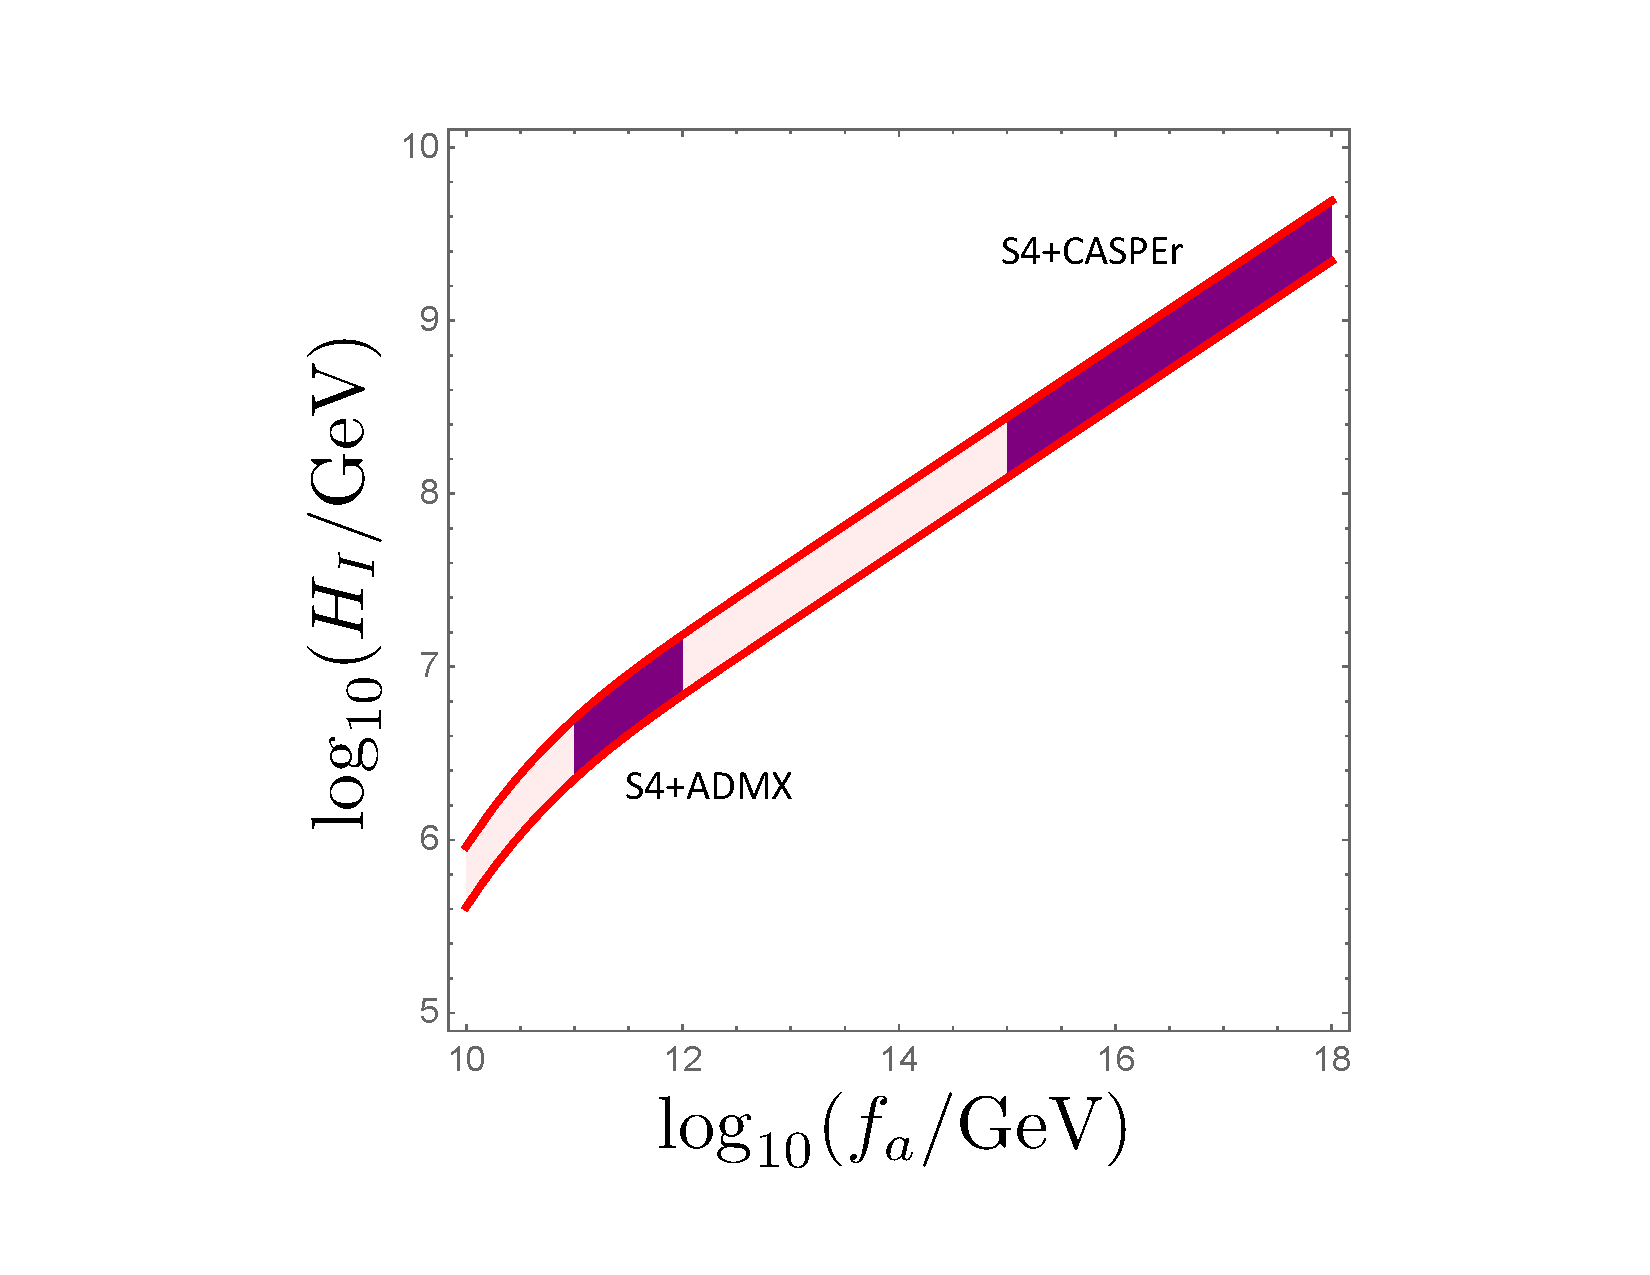
\includegraphics[width=0.4\textwidth]{Inflation/admx_casper_labelled.pdf} &
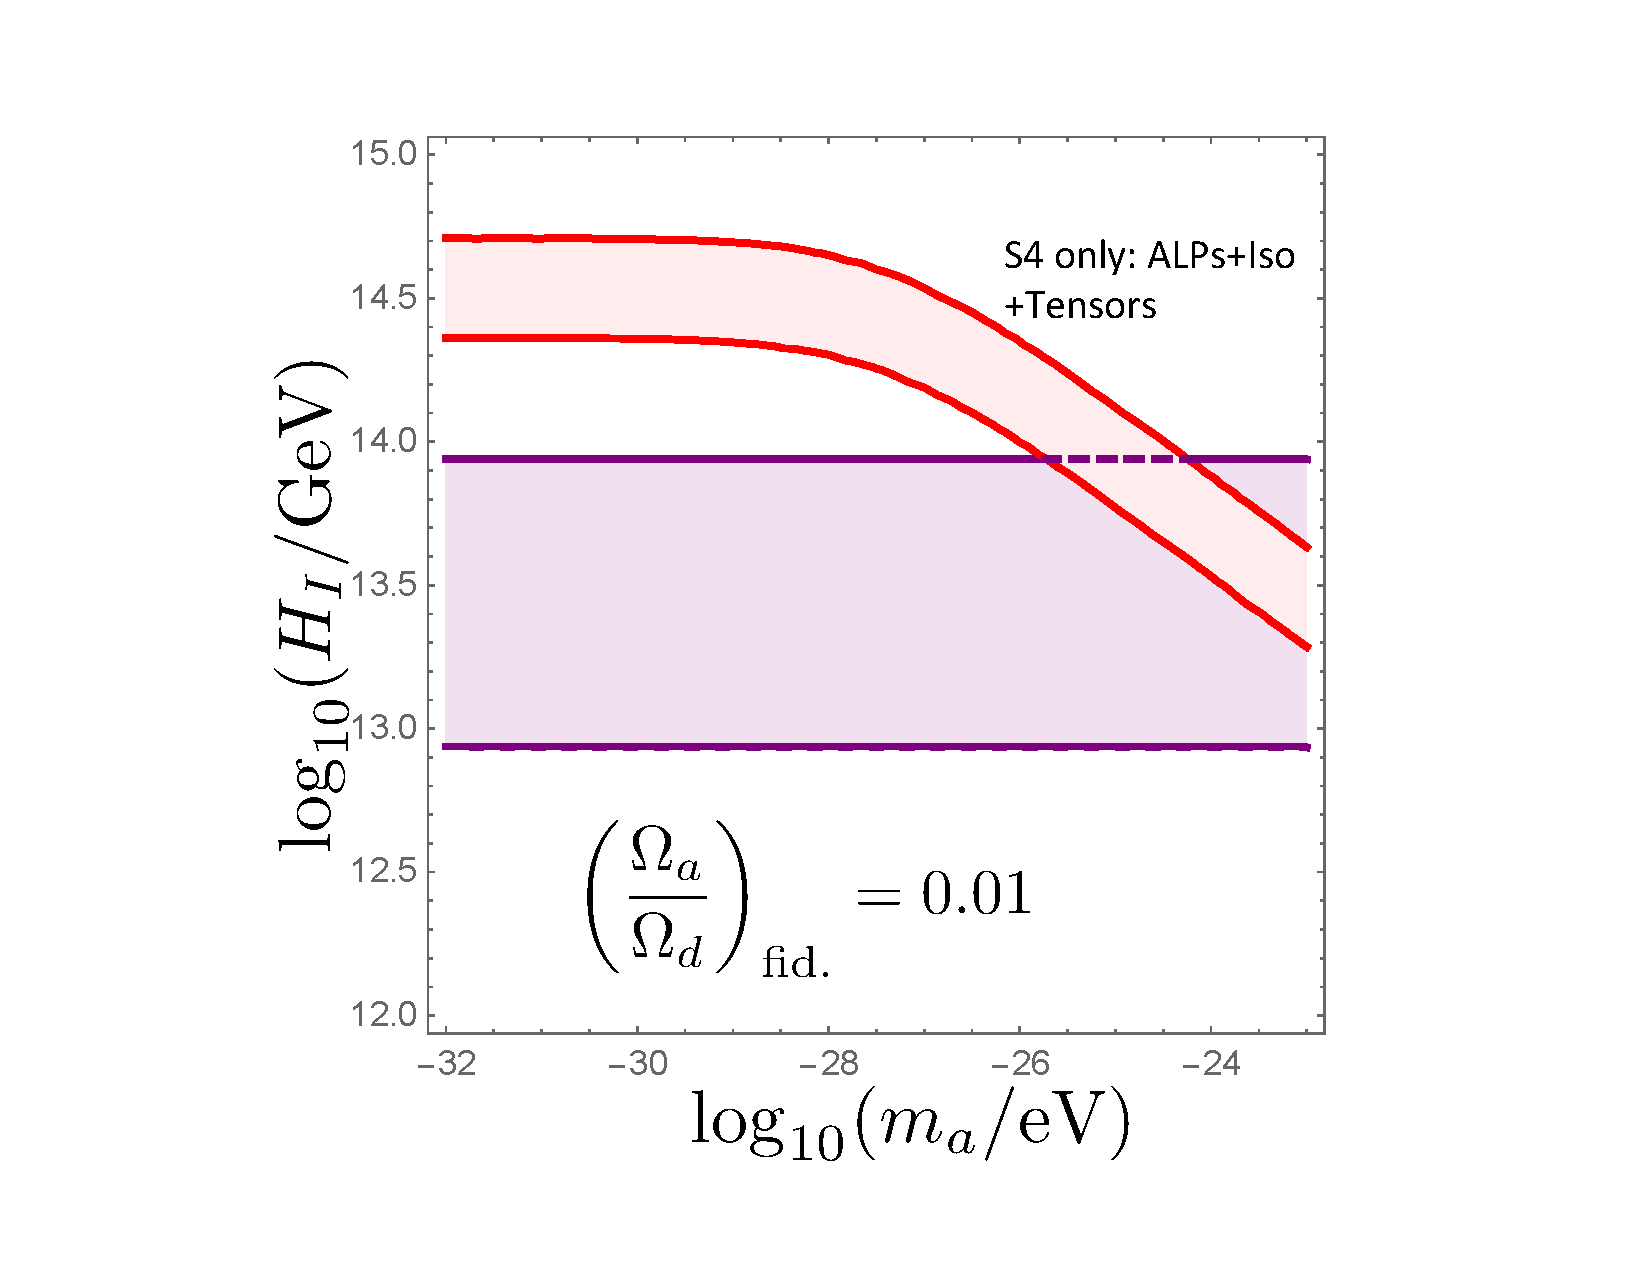
\includegraphics[width=0.4\textwidth]{Inflation/alp_iso_labelled.pdf}
 \end{array}$
 \end{center}
 \caption{Axion dark matter isocurvature. Red bands shows isocurvature amplitude consistent with \emph{Planck} and detectable with S4. \emph{Left Panel} The QCD axion: measuring the energy scale of inflation with S4+axion direct detection. Here we restrict axions to be all of the DM. The purple regions show the range of $f_a$ accessible to axion direct detection experiments. Combining ADMX~\cite{Asztalos:2009yp} (in operation), CASPEr~\cite{Budker:2013hf} (proposed), and S4 it is possible to measure $4\times 10^5\lesssim H_I/\text{GeV}\lesssim 4\times 10^9$. \emph{Right Panel} ALPs: a combination measurement using S4 alone. Assuming 1\% of the total DM resides in an ultralight axion, the mass and axion density can be determined to high significance using, for example, the lensing power. The isocurvature amplitude can also be determined, allowing for an independent determination of $H_I$ in the same regime as is accessible from tensor modes (purple band).}
\label{fig:qcd_isocurvature}
\end{figure*} 
We now consider isocurvature in ultralight ALPs (ULAs, see e.g. Refs.~\cite{Marsh:2013taa,Marsh:2014qoa}). ULA DM has a number of distinctive features in large scale structure and the CMB~\cite{Hlozek:2015axa,Marsh:2013ywa}. For ULAs with $10^{-32}\lesssim m_a/\text{eV}\lesssim 10^{-23}$ a DM fraction of $\Omega_a/\Omega_d$ in the range of 1\% is consistent with \emph{Planck}~\cite{Hlozek:2015axa} and high-$z$ galaxy formation~\cite{Bozek:2014uqa,Schive:2015kza}, yet can be distinguished from pure CDM using S4 lensing power at $>2\sigma$ (depending on the ULA mass, Sec.~\ref{sec:uladiabat}). Fig.~\ref{fig:qcd_isocurvature} (right panel) shows isocurvature constraints possible with S4, compared to tensor constraints. We fix the fiducial ULA fraction to 1\%, such that $\Omega_a$ and $m_a$ can be separately measured using the S4 lensing power, and thus using Eq.~(\ref{eqn:iso_amplitude}) a measurement of $A_I$ is a measurement of $H_I$. 

In contrast to the QCD axion, there are masses, $m_a\lesssim 10^{-26}\text{ eV}$, for which tensor modes impose a stronger constraint on $H_I$ than isocurvature (such that isocurvature in these ALPs would be undetectably small). However, there are also regions of overlap between possible tensor and isocurvature measurements. Using S4 in these regions, it is possible to make a combination measurement of isocurvature and axion parameters, giving an independent measurement of $H_I$:
\begin{equation} 2.5\times 10^{13}\lesssim H_I/\text{GeV}\lesssim 10^{14}\,
\text{(ultralight ALPs, S4 alone)}\,\,.
\end{equation}
This applies to ALPs in the mass range $10^{-26}\lesssim m_a/\text{eV}\lesssim 10^{-23}$, where effects on lensing of a 1\% axion fraction can be distinguished from CDM. \emph{Detecting isocurvature and lensing effects from ULAs using CMB-S4 can provide a measurement of $H_I$ complementary to searches for tensor modes.}%\footnote{We note that obtaining a 1\% fraction in such ALPs requires $f_a\gg 1.8\times 10^{13}\text{ GeV}$, and so isocurvature in ULA DM is guaranteed.}


\subsection{Constraints on Axion couplings}

%A ubiquitous component of extensions of the Standard Model are axions and/or axion-%like particles (ALPs).  Axions have been introduced to solve the strong-CP problem~%\cite{Peccei:1977hh}, the hierarchy problem~\cite{Graham:2015cka}, and the %naturalness problem of inflation~\cite{Freese:1990rb}.  Furthermore, they appear %generically in string theory in large numbers, leading to the qualitative phenomena %described as the string axiverse~\cite{Arvanitaki:2009fg}.

%ALPs typically appear as (pseudo)-Goldstone bosons of some high energy global %symmetry.  At low energy, the mass of the ALP is protected by an approximate shift %symmetry of the general form $a \to a + c$ where $a$ is the axion and $c$ is a %constant (for non-abelian Goldstone bosons, this transformation will include higher %order terms in $a$).  We will define an ALP to be any (pseudo)-scalar particle for %which all couplings to the Standard Model respect such a symmetry.  This symmetry %may be softly broken with an explicit mass term, although this is highly restricted %in the case of the QCD axion.

Two couplings of particular interest for axion phenomenology are the coupling to gluons and photons, 
\beq
\frac{1}{4} g_{a \gamma \gamma} a \tilde F_{\mu \nu}F^{\mu\nu} \ , \qquad \qquad \frac{1}{4} g_{a g g} a \tilde G_{\mu \nu}G^{\mu\nu}  \ .
\eeq
These couplings typically appear as the consequence of chiral anomalies.  The coupling of the axion to gluons is what makes the solution to the strong-CP problem possible.  The coupling to photons is somewhat model dependent but typically arises in conjunction with the gluon coupling.  In addition to or instead of these couplings, a variety of other possible couplings to matter may also be included.

\begin{figure}[h!]
\centering 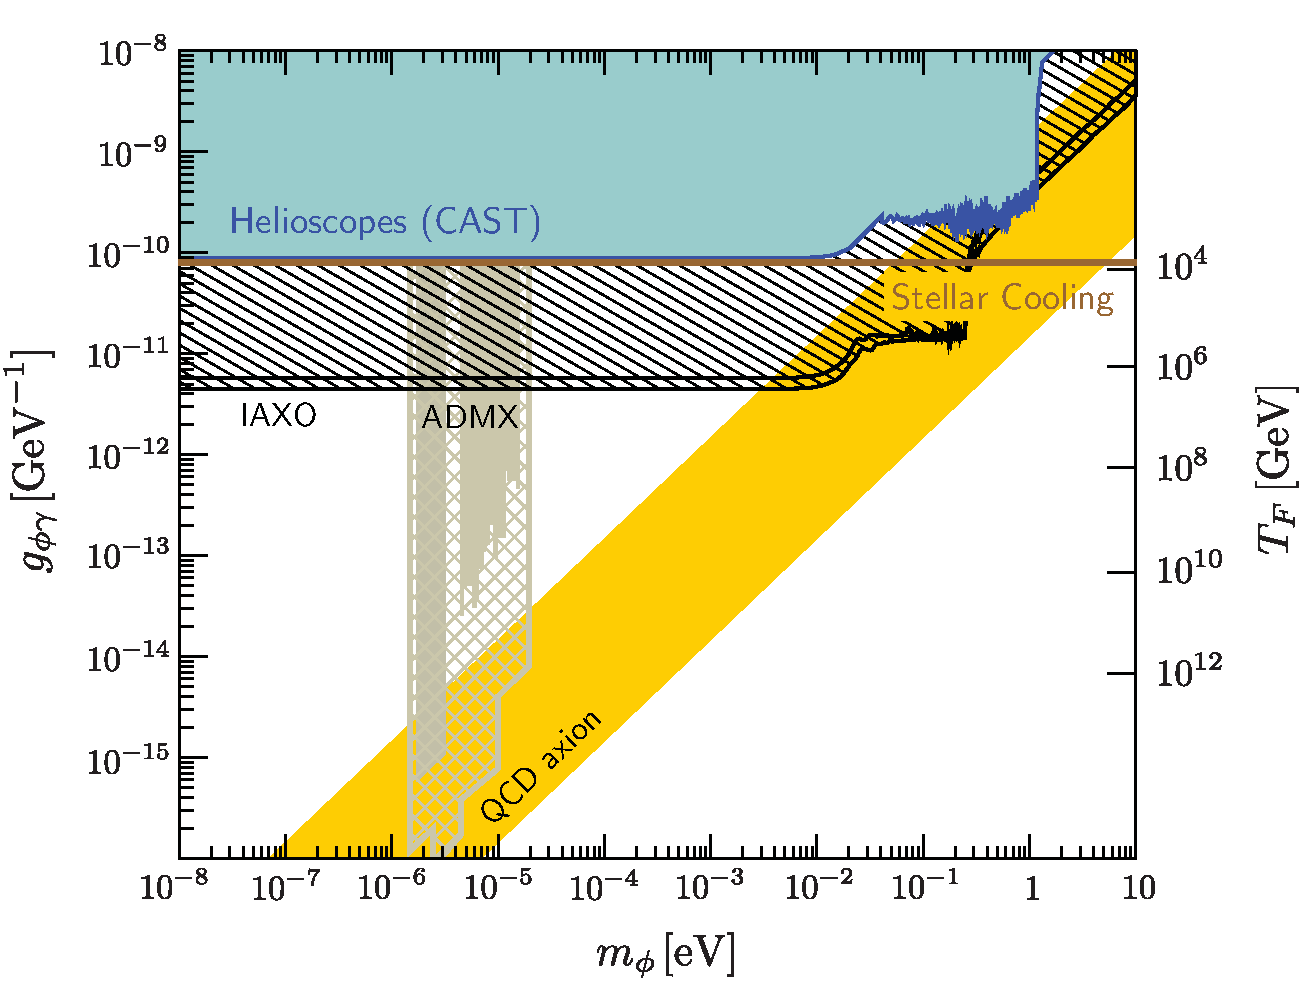
\includegraphics[width=0.70\textwidth]{Neutrinos/AxionPhotonWithFuture.pdf}
\caption{Relationship between freeze-out temperature ($T_F$) and axion-photon coupling ($g_{a\gamma\gamma}$).  While freeze-out is independent of the mass, experimental probes of the coupling are strongly mass dependent.  For $T_F > 10^4$~GeV the axion coupling would predict $\Delta \Neff = 0.027$.  Sensitivity to $\Delta\Neff$ at that level would translate into sensitivity to axions with $T_F \leq T_{\rm reheat}$.  For plausible values of $T_{\rm reheat} > 10^{10}$~GeV, cosmology is orders of magnitude more sensitive than existing bounds over a wide range of masses.}
\label{fig:axionphoton}
\end{figure}

Two very common features of models containing ALPs are that the ALPs are typically light (in many cases, $m \ll 1$~eV) and their interactions are suppressed by powers of the (typically large) decay constant $f_a$.  These two features make ALPs a particularly compelling target for cosmology (and $\Neff$ specifically).  Because of the small masses, they will often behave as relativistic species in the early universe.  Furthermore, because their production rate will scale as $T^{2n +1} / f_a^{2n}$ for some $n \geq 1$, they are likely to be thermalized at high temperatures.  Given that $\Delta \Neff > 0.027$ under such circumstances, a CMB experiment with sensitivity at this level will be sensitive to a very wide range of ALP models.

The coupling of axions to matter has an additional feature that it can bring axions into thermal equilibrium at low temperatures.  Specifically, the lowest dimension coupling of an axion to charged matter takes the form
\beq
{\cal L} = -\frac{\partial_\mu a}{\Lambda_\psi}  \bar \psi_i ( \gamma^\mu g^{ij}_V + g_A^{ij} \gamma^5 ) \psi_j
\eeq
where $\psi_{i}$ is any of the charged fermions of the Standard Model and $i,j$ label the three generations of fermions of with the same charges.  Above the scale of electroweak symmetry breaking (EWSB), this coupling leads to an abundance of axions with $\Delta \Neff = 0.027$.  Through freeze-out, we are again very sensitive to $g_V$ and $g_A$ at levels that vastly exceed current limits.  In addition, below the scale of EWSB, this coupling can bring the axions into thermal equilibrium at low temperatures (freeze-in) below the mass of the heaviest fermion, $T_F \lesssim m_{3}$.  Freeze-in will produce $\Delta \Neff \approx 0.05$ and is therefore easier to detect.  For reheating temperatures well above the electroweak scale, the sensitivity of freeze-out exceeds that of freeze-in, although both are far more sensitive than current limits on axion couplings to  second and third generation fermions.

The coupling to matter is motivated also by the approximate $U(3)^5$ flavor symmetry of the Standard Model.  It is natural for such couplings to arise if the axion is a goldstone boson that results from spontaneous breaking of this symmetry (or a sub-group).  Given the non-abelian nature of the flavor symmetry, these scenarios can often lead to many axions (also known as familons).  Under such circumstances, the contribution to freeze-out is given by 
\beq
\Delta \Neff = N_a \times 0.027
\eeq
where $N_a$ is the number of axions / number of broken generators of the symmetry group.  It is easy to find scenarios where $N_a\sim {\cal O}(10)$ which is at the current level of sensitivity.


{\it Status of current observations} -- Current constraints on ALPs arise from a combination of experimental~\cite{Graham:2015ouw}, astrophysical~\cite{Raffelt:2012kt}, and cosmological~\cite{Marsh:2015xka} probes.  Current cosmological constraints are driven by several effects that depend on the mass of the axion.  For axion masses greater than 100 eV, stable thermal ALPs are easily excluded because they produce dark matter abundances inconsistent with observations.  By including the free-streaming effects of thermal QCD-axions,  Planck data~\cite{DiValentino:2015wba} combined with local measurements provide the constrain $m_a < 0.525$ eV (95 \% CL).  At larger masses, ALPs become unstable and can be constrained by the change to $\Neff$ from energy injection as well as from spectral distortions and changes to BBN~\cite{Cadamuro:2011fd,Follin:2015hya}.

{\it Implications for CMB Stange IV} -- Sensitivity to $\Delta \Neff =0.027$ is sufficient to probe the entire mass range of ALPs down to $m_a =0$ under the assumption that it thermalized in the early universe.  Interpreting such bounds in terms of the couplings of axions is more complicated~\cite{Brust:2013xpv} and can depend on assumptions about the reheating temperature.  For high (but plausible) reheat temperatures of $10^{10}$ GeV, CMB stage IV would be sensitive to $g_{a\gamma \gamma}, \, g_{a g g} \,  < \, 10^{-13} {\rm GeV}^{-1}$~\cite{Baumann:2016wac} as illustrated in figures~\ref{fig:axionphoton} and~\ref{fig:axiondipole}.  These projected limits exceed current constraints and future probes for a range of possible axion masses (including the QCD axion).

The implications for the couplings to matter are similar for the contribution from freeze-out.  However, the freeze-in contribution of $\Delta \Neff \gtrsim 0.05$ would be easier to exclude experimentally, but still produces the limits~\cite{Baumann:2016wac}
\beq
\Lambda_{\psi_i}  \ >\ \left\{ \begin{array}{ll} \displaystyle 1.3\times 10^8 \, {\rm GeV} \left(\frac{g_{*,i}}{g_{*,\tau}}\right)^{\!-1/4} \left(\frac{m_i}{m_\tau}\right)^{\!1/2} & \quad i=\text{leptons}, \\[10pt]
\displaystyle 2.1\times 10^9 \, {\rm GeV} \left(\frac{g_{*,i}}{g_{*,t}}\right)^{\!-1/4} \left(\frac{m_i}{m_t}\right)^{\!1/2} & \quad i=\text{quarks}.
\end{array} \right.
\eeq
where $g_{*,i}$ is the number of degrees of freedom at temperature $T = m_i$.  For second and third generation fermions, these limits would exceed current bounds by several orders of magnitude.


\begin{figure}[h!]
\centering 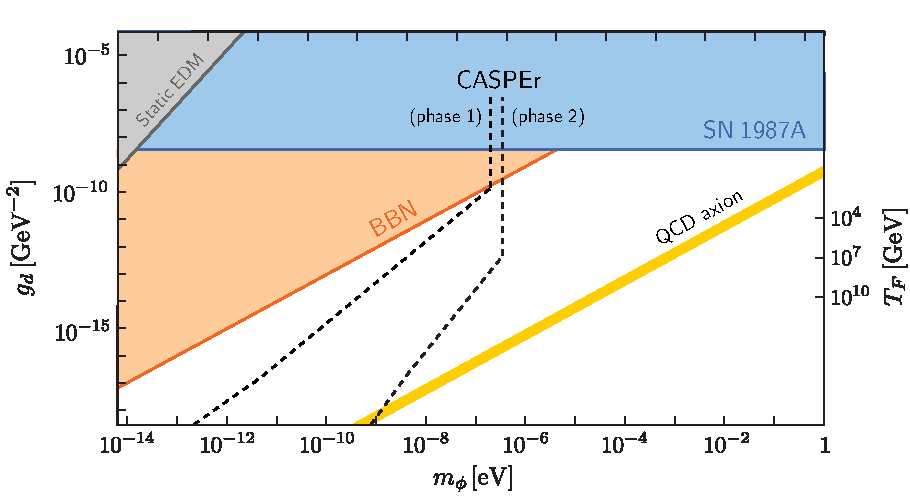
\includegraphics[width=0.70\textwidth]{Neutrinos/DipoleWithCASPErAndBBN.pdf}
\caption{Relationship between freeze-out temperature ($T_F$) and axion-gluon coupling via the neutron dipole ($g_d$).  While freeze-out is independent of the mass, experimental probes of the coupling are strongly mass dependent. We see that cosmology is more sensitive than current limits even for freeze-out temperatures below the eletro-weak phase transition and therefore could be probed by $\Delta \Neff > 0.027$.   }
\label{fig:axiondipole}
\end{figure}


\section{Neutrino constraints on BSM physics}

We primarily detect neutrinos in cosmology through their gravitational influence.  Light relics can contribute to the same observables, $\sum m_\nu$ and $\Neff$, and therefore these measurements constrain additional light degrees of freedom.  The precise relation between these observables and the underlying models depends on spin.  This section is organized by the spin of the relevant light particle from axions (spin 0) to gravitons (spin 2).  


\subsection{Sterile Neutrinos}
\label{sec:sterile_neutrinos}

\textcolor{red}{(DG:  Needs more basic introduction.  What is a sterile neutrino (include lagrangian) and how does it explain these anomalies?)}

A number of recent neutrino oscillation experiments have reported anomalies
that are possible indications of four or more neutrino mass eigenstates. The
first set of anomalies arose in short baseline oscillation experiments.
First, the Liquid Scintillator Neutirno Detector (LSND) experiment observed
electron antineutrinos in a pure muon antineutrino
beam \cite{Athanassopoulos:1997pv}. The MiniBooNE Experiment also observed
an excess of electron neutrinos and antineutrinos in their muon
neutrino beam \cite{Aguilar-Arevalo:2013pmq}. Two-neutrino oscillation
interpretations of these results indicate mass splittings of $\Delta m^2
\approx 1\rm\ eV^2$ and mixing angles of $\sin^2 2\theta \approx
3\times 10^{-3}$ \cite{Aguilar-Arevalo:2013pmq}. Another anomaly
arose from re-evaluations of reactor antineutrino fluxes that
indicate an increased flux of antineutrinos as well as a lower
neutron lifetime and commensurately increased the antineutrino events
from nuclear reactors by 6\%. This caused previous agreement of
reactor antineutrino experiments to have a $\sim$6\% deficit
\cite{Mention:2011rk,Huber:2011wv}. Another indication consistent with
sterile neutrinos was observed in radio-chemical gallium experiments for solar
neutrinos. In their calibrations, a 5-20\% deficit of the measured
count rate was found when intense sources of electron neutrinos from
electron capture nuclei were placed in proximity to the
detectors. Such a deficit could be produced by a $>1\rm\ eV$ sterile
neutrino with appreciable mixing with electron neutrinos
\cite{Bahcall:1994bq,Giunti:2010zu}. Some simultaneous fits to the
short baseline anomalies and reactor neutrino deficits, commensurate
with short baseline constraints, appear to prefer at least two extra
sterile neutrino states \cite{Conrad:2012qt,Kopp:2013vaa}, but see
Ref.~\cite{Giunti:2015mwa}. Because such neutrinos have relatively
large mixing angles, they would be thermalized in the early universe
with a standard thermal history, and affect primordial nucleosynthesis
\cite{Abazajian:2002bj} and CMB measurements of $\Neff$.

In addition, there are combinations of CMB plus LSS
datasets that are in tension, particularly with a smaller amplitude of
fluctuations at small scale than that inferred in zero neutrino mass
models. This would be alleviated with the
presence of massive neutrinos, extra neutrinos, or both. In particular,
cluster abundance analyses \cite{Wyman:2013lza,Ade:2015fva} and weak lensing analyses
\cite{Battye:2013xqa} indicate a lower amplitude of
fluctuations than zero neutrino mass \cite{Giusarma:2014zza}. Baryon Acoustic
Oscillation measures of expansion history are affected by the presence
of massive neutrinos, and nonzero neutrino mass may be indicated 
\cite{Beutler:2014yhv}, though 2015 Planck results show a lack of such
alleviation in cases with massive or extra neutrinos
\cite{Ade:2015xua}. 

There is a potential emergence of both laboratory and cosmological
indications of massive and, potentially, extra neutrinos. However, the
combined requirements of the specific masses to produce the short
baseline results, along with mixing angles that require thermalized
sterile neutrino states, are inconsistent at this point with
cosmological tension data sets
\cite{Joudaki:2012uk,Archidiacono:2013xxa}. The tension data sets are
not highly significant at this point ($\lesssim 3\sigma$), and there
are a significant set of proposals for short baseline oscillation
experiment follow up \cite{Abazajian:2012ys}. Future high-sensitivity
probes of neutrino mass and number such as CMB-S4 will be able to
definitively test for the presence of extra neutrino number and mass
consistent with sterile neutrinos.


\subsection{Light Fermions and Vectors}

A general approach to interpreting $\Neff$ constraints in terms of massless fields of arbitrary spin was undertaken in~\cite{Brust:2013xpv}.  One identifies the symmetry that is required to explain  the small mass of the particle, and then writes the most general interactions with the Standard Model consistent with the symmetry.  The couplings will take the form
\beq
{\cal L} \supset \sum_{\Delta_h, \Delta_s} \frac{1}{\Lambda^{\Delta_h+ \Delta_s-4}} \,  {\cal O}_{h, \Delta_h} \cdot {\cal O}_{s, \Delta_s}
\eeq
where ${\cal O}_{h,\Delta_h}$ is an operator of dimension $\Delta_h$ constructed only from hidden sector fields (and similarly for ${\cal O}_{s, \Delta_s}$ and Standard Model fields).  The total operator must be a scalar under both the Lorentz transformations and the symmetry that protects the mass of the hidden sector field(s).  The bounds on axions discussed in Section~\ref{sec:axions} are one such example, where the axion is protected by a shift symmetry.  For the purpose of this discussion, we have classified all scalars of this type as axions.

For a single Weyl fermion, $\chi$, the leading couplings to the Standard Model are through the anapole moment and four-fermion interactions
\beq
{\cal L} \supset \frac{\chi^{\dagger} \bar \sigma^{\mu} \chi}{\Lambda_{\chi}^2} \Big( d_a  \, \partial^\nu F_{\mu \nu} + d_f \,  \bar \psi \gamma_\mu \psi \Big) \ ,
\eeq
where we have chosen a chosen one of several four-fermion interactions for illustration and $d_f, d_a$ are order one numbers.  Current experimental constraint from LEP and the LHC limit $\Lambda_\chi \gtrsim \, 1$ TeV.  Similar bounds are set by Planck by excluding the contributions to $\Delta \Neff$ from freeze-out after the QCD phase transition.  If we are sensitive to the minimal contribution from a Weyl fermion of $\Delta \Neff = 0.047$, then for a reheat temperature of $T_{\rm reheat} \sim 10^{10}$ GeV, we would be sensitive to $\Lambda_\psi \lesssim 10^{12}$ GeV.  We see that for an order of magnitude improvement in sensitivity to $\Neff$, we get as much as a nine order of magnitude improvement in sensitivity to $\Lambda_\psi$.  

For a hidden Dirac fermion, $X$, the leading coupling is through an effective dipole interaction.  A similar interaction also permits a hidden $U(1)$ gauge boson, $A'_\mu$, to couple to Standard Model fermions.
\beq
{\cal L} \supset  \frac{1}{\Lambda_X} \bar X \sigma_{\mu\nu} X  F^{\mu \nu} + \frac{1}{\Lambda_{A'}^2} H \bar \psi \sigma_{\mu\nu} \psi  F'_{\mu \nu}  \ ,
\eeq
where $F'_{\mu \nu}$ is the field strength of $A'_\mu$.  We have included the Higgs field, $H$, in the coupling to Standard Model fermions as it is required by gauge invariance above the scale of EWSB.  Stellar cooling provides a strong constraint of $\Lambda_X \gtrsim 10^9$ GeV and $\Lambda_{A'} \gtrsim 10^5$ GeV.  

Freeze-out above the scale of EWSB for a Dirac fermion produces $\Delta \Neff = 0.094$ and $\Delta\Neff = 0.054$ for a hidden photon.  For a reheating temperature of $10^{10}$ GeV, we are sensitive to $\Lambda_X \lesssim 10^{13}$ GeV and $\Lambda_{A'}  \lesssim 10^{11}$ GeV respectively.  The Dirac fermion will be accessible with CMB Stage IV and will improve on the stellar cooling constraint for a reheat temperature $T_{\rm reheat} > 10^4$ GeV.

\subsection{Gravitinos}

One of the most popular extensions of the Standard Model is supersymmetry, which is motivated both by naturalness and gauge coupling unification.  Although the most generic possibilities are under significant tension for the LHC, there are still a variety of possibilities consistent with low-scale supersymmetry.

One of the universal predictions of supersymmetry is the existence of a spin-3/2 partner to the graviton, the gravitino.  The gravitino mass is determined by the absolute scale of supersymmetry breaking, 
\beq
m_{\frac{3}{2}} = \frac{|F|}{\sqrt{3} M_{\rm pl}}
\eeq
where $|F|$ is the order parameter for the scale of SUSY breaking (the vacuum expectation value of the auxiliary field $F$).  This result does not depend on details of the mechanism of SUSY breaking unlike the super-partners of the rest of the Standard Model particles.

The typical coupling strength of the gravitino is the same as the graviton, $8 \pi G = \Mpl^{-2}$.  However, the strength of the coupling to the helicity-1/2 component of the gravitino is enhanced by $\Mpl^2 /F$.  This is simply the statement that the goldstino of SUSY breaking is coupled with strength $F^{-1}$ (but is `eaten' by the gravitino).  Due to the enhanced coupling, the gravitino can be in thermal equilibrium with the Standard Model at plausible temperatures in the early universe.  The gravitino therefore behaves just like a Weyl fermion in figure~\ref{fig:Neff_thermal}.

For $m_{3/2} \lesssim 10$ eV, hot relic gravitinos free stream on the scale of the CMB and therefore lead to observable signatures.  Current data from Planck already requires that $m_{3/2} < 4.7$ eV from a combination of the primary CMB and CMB lensing~\cite{Osato:2016ixc}.  To probe lower masses, note that for $m_{3/2} < {\cal O}(1)$ eV a gravitino will behave as free-streaming radiation from the point of view of the CMB.  One finds that for these low values of the mass, gravitinos contribute a shift to $\Neff$,
\beq
\left(\Delta \Neff\right)_{3/2} \, \gtrsim \, 0.057 \ .
\eeq
At $\sigma(\Neff) \sim 0.03$, CMB Stage IV can rule out all low-scale SUSY breaking models allowed by current cosmology.  

\subsection{Gravitational Waves}\label{sec:constraintsntNeff}

Since gravitational waves are massless and free-streaming, any gravitational waves which were present in the early universe naturally contribute to the total radiation energy density, and can therefore be constrained with $\Neff$ \cite{Boyle:2003km,Boyle:2007zx,Stewart:2007fu,Meerburg:2015zua,Lasky:2015lej}.

Let us briefly review how to compute the energy density of a stochastic background of gravitational waves, following the treatment of \cite{Isaacson:1968zza,Misner:1974qy,Watanabe:2006qe,Maggiore:1900zz}.  We will take the metric of spacetime to be given by a background component $\bar{g}_{\mu}$ described by the flat Friedmann-Robertson-Walker metric and a perturbation $\delta g_{\mu\nu}$.  We will take the characteristic frequency of $\delta g_{\mu\nu}$ to be much higher than that of $\bar{g}_{\mu\nu}$.  In particular, we will focus on gravitational waves whose wavelengths are much shorter than scales of cosmological interest.

The Ricci tensor can be expanded in powers of $\delta g$ as
\begin{equation}\label{eq:Ricci_GW}
	R_{\mu\nu} = \bar{R}_{\mu\nu} + R_{\mu\nu}^{(1)} + R_{\mu\nu}^{(2)} + \cdots \, .
\end{equation}
We are interested in determining how spacetime is curved by the presence of small scale gravitational waves, or in other words, how $\bar{R}_{\mu\nu}$ is affected by terms containing $\delta g_{\mu\nu}$.  Since $R_{\mu\nu}^{(1)}$ is linear in $\delta g_{\mu\nu}$, it contains only high frequency components, while on the other hand, $R_{\mu\nu}^{(2)}$ has both low and high frequency parts.  

The high frequency part of Einstein's equations governs how gravitational waves propagate in a curved background, and is not necessary here.  For the low frequency part, we can take an average over several cycles of the high frequency modes, which then gives
\begin{equation}\label{eq:Einstein_Eq_GW}
	\bar{R}_{\mu\nu} = -\left\langle R_{\mu\nu}^{(2)}\right\rangle + 8\pi G \left\langle T_{\mu\nu}-\frac{1}{2}g_{\mu\nu}T\right\rangle \, .
\end{equation}
We can then read off the effective energy-momentum tensor of small scale fluctuations
\begin{equation}\label{eq:EM_Tensor_GW}
	T_{\mu\nu}^\mathrm{GW} = -\frac{1}{8\pi G} \left \langle R_{\mu\nu}^{(2)}-\frac{1}{2}\bar{g}_{\mu\nu}R^{(2)} \right\rangle + \mathcal{O}(\delta g^3) \, .
\end{equation}
If we take our perturbation to be of the form $\delta g_{ij} = a^2 h_{ij}$ with $h_{ij,j} = 0$ and $h_{ii} = 0$, we can compute the energy density of gravitational waves explicitly in the transverse traceless gauge
\begin{equation}\label{eq:Energy_GW}
	\rho_\mathrm{GW} = T_{00}^\mathrm{GW} = \frac{1}{32 \pi G}\delta^{ik}\delta^{j\ell}\left\langle \dot{h}_{ij} \dot{h}_{k\ell} \right\rangle + \mathcal{O}(\delta g^3) \, .
\end{equation}

We will define the gravitational wave power spectrum as
\begin{equation}\label{eq:GW_power_spectrum}
	\left\langle h_{ij}(\eta,\mathbf{x})h^{ij}(\eta,\mathbf{x})\right\rangle \equiv \int  d \log k \, \mathcal{P}_t(k) \left[\mathcal{T}(\eta,k)\right]^2 \, ,
\end{equation}
where $\mathcal{P}_t(k)$ is the primordial power spectrum of gravitational waves and $\mathcal{T}(\eta,k)$ is the tensor transfer function.  The energy density of gravitational waves is then given by
\begin{equation}\label{eq:GW_energy_density}
	\rho_\mathrm{GW} = \frac{1}{32\pi G a^2}\int  d\log k \, \mathcal{P}_t(k) \left[\mathcal{T}'(\eta,k)\right]^2 \, ,
\end{equation}
where the prime denotes a derivative with respect to conformal time $\eta$.

Direct searches for the stochastic gravitational wave backgound are often quoted in terms of the normalized energy density per logarithmic scale
\begin{equation}\label{eq:Omega_GW}
	\Omega_\mathrm{GW}(k) \equiv \frac{8\pi G}{3H_0^2}\frac{d\rho_\mathrm{GW}}{d\log k} = \frac{\mathrm{P}_t(k)}{12H_0^2a_0^2} \left[\mathcal{T}'(\eta_0,k)\right]^2 \, .
\end{equation}
On the other hand, constraints on $\Neff$ provide an integral constraint on the spectrum of gravitational waves since waves of all frequencies contribute to the total energy density.

If for example, we take the primordial gravitational wave power spectrum to be a simple power law of the form $\mathcal{P}_t(k) = A_t \left(\frac{k}{k_\star}\right)^{n_t}$ (as in Eq.~(\ref{eq:power_spectra_power_law})), we can use a constraint on $\Neff$ to place bounds on the tensor spectral tilt $n_t$.  The contribution to $\Neff$ can then be approximated for $n_t>0$ as \cite{Meerburg:2015zua}
\begin{equation}\label{eq:Neff_GW}
	\Delta \Neff \simeq \left(3.046 + \frac{8}{7}\left(\frac{11}{4}\right)^{4/3}\right)\frac{A_t}{24n_t}\left(\frac{k_\mathrm{UV}}{k_\star}\right)^{n_t} \, ,
\end{equation}
where $k_\mathrm{UV}$ represents the ultraviolet cutoff of the primordial tensor power spectrum.  While this constraint does not probe the regime of great interest for inflationary models, it does provide a useful constraint on early universe alternatives to inflation which predict positive tensor tilt.


\section{Microwave Background Anomalies}

Several unexpected features have been observed in the temperature of the CMB sky at relatively low-l or large angular scales.  Some of these were first noticed in COBE data,  
and all have been seen in both WMAP and Planck maps.  These include: 
\begin{itemize}
  \item a lack of correlation on the largest angular scales;
  \item alignment of the lowest multipole moments with one another and with the geometry and motion of the Solar System;
 \item greater power in odd-parity modes than in even-parity ones;
  \item a hemispherical asymmetry or dipolar modulation of the power.
\end{itemize}

Compared to the expectations of the best-fit inflationary $\Lambda$CDM model, the individual p-values of these features are in the per mille to per cent level, and therefore each anomaly has a frequentist probability at approximately the 3-sigma level or higher.  Since certain pairs of anomalies are uncorrelated in $\Lambda$CDM, in combination they nominally represents a very significant detection of anomalous behaviour. 

There are however two possible concerns before one can conclude that the CMB large-angle pattern is truly anomalous. First, these features were identified a posteriori and are characterized by statistics that were devised after the anomalies were first noted. Second, there is no physical understanding of how the collection of such features could arise. In order to help address or resolve these concerns, it is therefore crucial to obtain additional information about the large-scale primordial fluctuations, and to devise a successful model or other explanation.

The observed features can have two possible origins: either our cosmological model is incomplete and requires a modification (the “new physics hypothesis”), or we just happen to live in a realization of that model that is statistically unlikely (the “fluke hypothesis”).   Meanwhile, cosmologists have effectively exhausted their ability to obtain further independent CMB temperature data that can test these anomalies, as observations are already cosmic-variance limited at the relevant angular scales.

It has been suggested that one may nevertheless make observational progress even in the absence of an alternative model.  This can occur in two ways:
\begin{enumerate}
  \item In the fluke hypothesis the conditional probability distributions of $\Lambda$CDM for correlation functions of CMB polarization
  (and other observables) with CMB temperature and with one another are altered by the observed temperature anomalies  
  (Dvorkin et al 2008, Copi et al 2013, Yoho et al. 2013). 
  \item In the new physics hypothesis, a given phenomenological model that explains the anomalies will have observational consequences
  for other observable quantities [Yoho et al. 2015]. For example, the absence of large-angle correlations in T may reflect a lack of
  long-distance correlation in a fundamental physical quantity like the potential; similarly, 
  a hemispherical asymmetry in TT power could cause a similar asymmetry in EE.
\end{enumerate}

A variety of ideas have been proposed to explain the anomalies, ranging from Solar system dust artifacts to anisotropic models of inflation (for a summary, see Copi et al, 2016). Unfortunately, none of those ideas lead to a convincing explanation, as it is simply difficult to find models that explain the alignments of the largest primordial structures in the universe while at the same time lowering the amplitude of large-angle temperature correlations (e.g. Gordon et al, 2005). 

Additional information from polarization would be of great help. To address the first three anomalies we list above would probably require a space mission, due to the need to access very low $\ell$. But CMB-S4 can shed light on the fourth one. 

CMB-S4, alone or in combination with other data, can begin to explore both the cosmological and the fluke explanation for the hemispherical power asymmetry.  For example, $\Lambda$CDM instructs us how to remove the part of the E-mode signal that is correlated to temperature; the remainder should be Gaussian random and statistically isotropic.  If it contains a hemispherical anomaly (especially one aligned with the temperature asymmetry), that would be evidence against the fluke hypothesis [Copi, Knox, O’Dwyer and Starkman, contribution to March 9/10 S4 meeting, in preparation]. 

\section{Cosmic Birefringence}
\textbf{More text to come from Vera}
The simplest dynamical way to model the accelerated expansion of the universe is to invoke a new slowly evolving scalar field that dominates its energy budget (the quintessence models for DE). Such a field generically couples to photons through the Chern-Simons term in the electromagnetic Lagrangian, causing linear polarization of photons propagating cosmological distances to rotate---the effect known as cosmic birefringence~\cite{1998PhRvL..81.3067C}. In the case of the CMB, such rotation converts the primordial E mode into B mode, producing characteristic TB and EB cross-correlations in the CMB maps \cite{2009PhRvL.102k1302K,2009PhRvD..80b3510G}. Even though there is no firm theoretical prediction for the size of this effect, if observed, it would be a clear “smoking-gun” evidence for physics beyond the standard model. Previous studies have used quadratic estimator formalism to constrain this effect \cite{2012PhRvD..86j3529G}, with the best current limit coming from sub-degree scale polarization measurements with POLARBEAR \cite{Ade:2015cao} ($<0.33$ deg$^2$ for the amplitude of a scale-invariant rotation-angle power spectrum). A promising way to pursue search for cosmic birefringence in the future is measurement of the off-diagonal EB cross correlations on small angular scales. {\bf Put in more specific predictions for S4?}

\section{Primordial Magnetic Fields}

The origin of the microgauss ($\mu$G) strength magnetic fields in galaxies and galaxy clusters is one of the long standing puzzles in astrophysics \cite{Durrer:2013pga}. It is challenging to explain such fields based solely on the dynamo mechanism, without there being some initial seed field. However, if magnetic fields were present in the early universe, they would remain frozen in the cosmic plasma and collapse with the rest of the matter to form the galactic fields \cite{Grasso:2000wj}, or at least provide the seeds for the dynamo. A primordial magnetic field (PMF) could be produced in the aftermath of cosmic phase transitions \cite{Vachaspati:1991nm} or in specially designed inflationary scenarios \cite{Turner:1987bw,Ratra:1991bn}. Detecting their signatures in the CMB temperature and polarization would decisively prove their primordial origin. Aside from explaining the galactic fields, bounds on PMF have profound implications for our understanding of the early universe.  They help constrain theories of inflation \cite{Bonvin:2011dt}, models of the QCD and electroweak phase transitions \cite{Caprini:2007xq} and baryogenesis \cite{Vachaspati:2001nb}.

A stochastic PMF affects CMB in several ways. Magnetic stress-energy induces scalar, vector and tensor mode perturbations in the metric, and the Lorentz force generates vorticity in the photon-baryon fluid \cite{Subramanian:1998fn,Mack:2001gc,Lewis:2004ef,Shaw:2009nf,Paoletti:2010rx}. Dissipation of PMF on small scales dumps energy into the plasma, which produces spectral distortions and affects the recombination history \cite{Kunze:2014eka}.  Finally, Faraday Rotation (FR) of CMB polarization converts some of the $E$-modes into $B$-modes \cite{Kosowsky:2004zh,Pogosian:2011qv}.

Stochastic PMF has two potentially observable frequency independent contributions to the $B$-mode spectrum \cite{Shaw:2009nf}. One comes from the passive, or uncompensated tensor mode, which is generated by the PMF before neutrino decoupling. For nearly scale-invariant PMF, the spectrum of this component is indistinguishable from the inflationary gravity wave signal. The amplitude of this tensor contribution is proportional to $B^4_{1\rm{Mpc}} [\ln(a_\nu / a_{\rm{PMF}})]^2$, where $B_{1\rm{Mpc}}$ is the PMF strength smoothed over $1$Mpc, $a_\nu$ is the scale factor at neutrino decoupling and $a_{\rm{PMF}}$ is the scale factor at which PMF was generated. The other is the PMF vector mode which peaks at $l \sim 2000$, with the precise peak position dependant on the PMF spectrum. The vector-mode contribution is independent of $a_{\rm{PMF}}$. 

Planck data limits the magnetic field strength to $B_{1 {\rm Mpc}}<4.4$ nanogauss (nG) at the $95\%$ confidence level \cite{Ade:2015cva}. Similar bounds were recently obtained by POLARBEAR \cite{Ade:2015cao} based on their B-mode spectrum alone.

\section{Cosmic Strings}

Cosmic strings can at most contribute O(1\%) to the total CMB temperature anisotropy~\cite{Ade:2013xla,Lizarraga:2014xza,Lazanu:2014eya}, however, they can still generate observable B-modes. As shown in \cite{Moss:2014cra}, the bounds on cosmic strings obtained solely from the POLARBEAR \cite{Ade:2014afa} and BICEP2  \cite{Ade:2014xna} B-mode spectra are comparable to those from temperature spectra. CMB-S4 polawill be able to reveal the presence of cosmic strings through their B-mode signature even if strings contribute as little as 0.1\% to the CMB temperature anisotropy \cite{Avgoustidis:2011ax}. 
\textbf{Renee Hlozek to add both text and plots/tables of constraints}


